
%% paper.tex
%% for ISORC 2016
%% 2016/11/29
%% by Takuro Yamamoto

\documentclass[conference]{IEEEtran/IEEEtran}
% Some Computer Society conferences also require the compsoc mode option,
% but others use the standard conference format.
%
% If IEEEtran.cls has not been installed into the LaTeX system files,
% manually specify the path to it like:
% \documentclass[conference]{../sty/IEEEtran}

% Package List
%\usepackage[dvips]{graphics}
\usepackage[dvipdfmx]{graphicx}
\usepackage{amssymb}
\usepackage{float}
\usepackage{enumerate,cite,url}
\usepackage{listings,jlisting}
\lstset{%
    language={c},%
    basicstyle={\footnotesize\ttfamily},%
    identifierstyle={\footnotesize},%
    commentstyle={\footnotesize\itshape},%
    keywordstyle={\footnotesize},%\bfseries},%
    ndkeywordstyle={\footnotesize},%
    stringstyle={\footnotesize\it},
    frame={tb},
    breaklines=true,
    columns=[l]{fullflexible},%
    numbers=left,%
    xrightmargin=0zw,%
    xleftmargin=3zw,%
    numberstyle={\scriptsize},%
    stepnumber=1,
    numbersep=1zw,%
    lineskip=-0.5ex%
}

% *** Do not adjust lengths that control margins, column widths, etc. ***
% *** Do not use packages that alter fonts (such as pslatex).         ***
% There should be no need to do such things with IEEEtran.cls V1.6 and later.
% (Unless specifically asked to do so by the journal or conference you plan
% to submit to, of course. )


% correct bad hyphenation here
\hyphenation{op-tical net-works semi-conduc-tor}


\begin{document}
%
% paper title
% Titles are generally capitalized except for words such as a, an, and, as,
% at, but, by, for, in, nor, of, on, or, the, to and up, which are usually
% not capitalized unless they are the first or last word of the title.
% Linebreaks \\ can be used within to get better formatting as desired.
% Do not put math or special symbols in the title.
\title{TINET+TECS: Component-Based TCP/IP Protocol Stack for Embedded Systems}


% author names and affiliations
% use a multiple column layout for up to three different
% affiliations
% \author{
% \IEEEauthorblockN{Takuro Yamamoto}
% \IEEEauthorblockA{Graduate School of Engineering Science\\Osaka University}
% \and
% \IEEEauthorblockN{Takuma Hara}
% \IEEEauthorblockA{Graduate School of Information Science\\Nagoya University}
% \and
% \IEEEauthorblockN{Takuya Ishikawa}
% \IEEEauthorblockA{Graduate School of Information Science\\Nagoya University}
% \and
% \IEEEauthorblockN{Hiroshi Oyama}
% \IEEEauthorblockA{OKUMA Corporation}
% \and
% \IEEEauthorblockN{Hiroaki Takada}
% \IEEEauthorblockA{Graduate School of Information Science\\Nagoya University}
% \and
% \IEEEauthorblockN{Takuya Azumi}
% \IEEEauthorblockA{Graduate School of Engineering Science\\Osaka University}
% }

% conference papers do not typically use \thanks and this command
% is locked out in conference mode. If really needed, such as for
% the acknowledgment of grants, issue a \IEEEoverridecommandlockouts
% after \documentclass

% for over three affiliations, or if they all won't fit within the width
% of the page, use this alternative format:
% 
\author{
\IEEEauthorblockN{
Takuro Yamamoto\IEEEauthorrefmark{1},
Takuma Hara\IEEEauthorrefmark{2},
Takuya Ishikawa\IEEEauthorrefmark{2}, 
Hiroshi Oyama\IEEEauthorrefmark{3},
Hiroaki Takada\IEEEauthorrefmark{2} and
Takuya Azumi\IEEEauthorrefmark{1}}
\IEEEauthorblockA{\IEEEauthorrefmark{1}Graduate School of Engineering Science, Osaka University}
\IEEEauthorblockA{\IEEEauthorrefmark{2}Graduate School of Information Science, Nagoya University}
\IEEEauthorblockA{\IEEEauthorrefmark{3}OKUMA Corporation}
}

% use for special paper notices
%\IEEEspecialpapernotice{(Invited Paper)}

% make the title area
\maketitle

\setcounter{topnumber}{5}       % ページ上部の図表は 5 個まで
\def\topfraction{1.00}          % ページの上 1.00 まで図表で占めて可
\setcounter{bottomnumber}{5}    % ページ下部の図表は 5 個まで
\def\bottomfraction{1.00}       % ページの下 1.00 まで図表で占めて可
\setcounter{totalnumber}{10}    % ページあたりの図表は 10 個まで
\def\textfraction{0.04}         % ページうち本文が占める割合の下限

% As a general rule, do not put math, special symbols or citations
% in the abstract
\begin{abstract}

% Embedded systems are applied to Internet of Things (IoT), and the high productivity of embedded network software is required.
High productivity embedded network software is required to run embedded systems within the Internet of Things (IoT).
Tomakomai InterNETworking (TINET) is a Transmission Control Protocol/Internet Protocol (TCP/IP) protocol stack for use in embedded systems.
Although TINET is a compact protocol stack, it comprises many complex source codes and is difficult to maintain, extend, and analyze.
To improve scalability and configurability, this paper proposes TINET componentized with the Toyohashi Open Platform for Embedded Real-time Systems (TOPPERS) embedded component system (TINET+TECS), a component-based TCP/IP protocol stack for embedded systems.
This component-based TINET offers software developers high productivity through variable network buffer sizes and the ability to add or remove TCP (or UDP) functionality.
TINET+TECS utilizes a dynamic TECS component connection method to satisfy the original TINET specifications.
The results of an experimental comparison between the proposed component-based and original TINETs show that the execution time and memory consumption overhead are reduced and the configurability is improved.

\end{abstract}

% no keywords

% For peer review papers, you can put extra information on the cover
% page as needed:
% \ifCLASSOPTIONpeerreview
% \begin{center} \bfseries EDICS Category: 3-BBND \end{center}
% \fi
%
% For peerreview papers, this IEEEtran command inserts a page break and
% creates the second title. It will be ignored for other modes.
\IEEEpeerreviewmaketitle

\section{Introduction}
\label{sec:Introduction}

The Internet of Things (IoT) is an essential next evolutionary step for the Internet \cite{par:IoTIndustries} \cite{par:IoTComputing} in which various items and platforms, for example, wearable devices, smart devices, and smart homes, will be connected via the Internet to further enrich people's lives.
However, as the IoT uses embedded systems such as data sensors and controlling actuators as elemental constituents, it is often not practical to implement the same Transmission Control Protocol/Internet Protocol (TCP/IP) protocol stacks used by traditional computing systems because embedded systems face restrictions in terms of, for example, low memory capacity.

Tomakomai InterNETworking (TINET) is a compact TCP/IP protocol stack for embedded systems \cite{url:TINET}.
As TINET supports functionalities such as a minimum copy frequency and the elimination of dynamic memory control, it requires significantly reduced memory for its TCP/IP protocol stack and is therefore suitable for embedded systems.
However, TINET comprises many complex source codes, i.e., it contains many files and defines many macros, which can be problematic for software developers seeking to maintain, extend, and analyze the software.
Thus, embedded network software is required for high productivity and quality.

One approach to improving software productivity is component-based development, a design technique that can be applied in reusable software development for embedded systems \cite{par:Crnkovic}\cite{par:CBD} such as TECS \cite{par:TECS} \cite{par:hr-tecs}, AUTOSAR \cite{url:AUTOSAR}, or SaveCCM \cite{par:SAVEapproach}.
Component-based systems are flexible to software extension and specification changes.

This paper proposes a component-based TCP/IP protocol stack for embedded systems--TINET componentized with the Toyohashi Open Platform for Embedded Real-time Systems (TOPPERS) embedded component system (TINET+TECS)--to improve the configurability and scalability of TCP/IP software.
Because it is a component system suitable for embedded systems, TECS \cite{par:TECS} \cite{par:hr-tecs} is used to componentize TINET in the proposed protocol stack.
As TECS supports static configurations that statically define component behaviors and interconnections, it can optimize the componentization overhead.

In addition to satisfying the original TINET specifications, the proposed framework utilizes the TECS dynamic connection capability to dynamically switch component bindings.
Although general TCP/IP protocol servers dynamically process requested ports, i.e., HTTP (port: 80) and HTTPS (port: 443), embedded systems are restricted in their dynamic processing ability owing to strict memory constraints.
TINET supports the static generation of Communication Endpoints (CEPs) and Reception Points (REPs), which are similar to sockets.
As TINET+TECS, like TINET, statically generates components and dynamically combines them in the same manner, TINET+TECS reduces the dynamic increase of memory consumption.

In the proposed framework, software applications can be developed using both TECS method and existing methods.
Software applications can be developed as TECS components because TINET+TECS is a component-based framework.
Furthermore, TECS supports the use of an adapter to call TECS component functions from non-TECS codes, which allows for the use of existing TCP/IP applications without modification.

This paper evaluates the overheads of execution time and memory consumption and the amount of code line changes needed to add and remove functionalities in order to improve configurability with small overheads.
Furthermore, the advantages of dynamic connection in terms of the memory consumption and low overhead of the TECS adapter are demonstrated.

{\bf Contributions:} This paper provides the following contributions:

\begin{enumerate}

    \item {\bf Improve configurability}\mbox{}\\
        Because TINET+TECS is a component-based system, its software can flexibly change as system's configuration by, for example, resizing network buffer, adding/removing TCP (or UDP) functionality, or supporting either IPv4 or IPv6.
        In addition, the use by TINET+TECS of individual component diagrams enables visualization of an entire system.

    \item {\bf Dynamic connection method}\mbox{}\\
        Dynamically switching the binding of components, that is, switching between a TINET communication endpoint and REP, realizes a TCP/IP protocol stack for an embedded system.
        
    \item {\bf Support legacy codes}\mbox{}\\
        TINET+TECS can be applied to existing applications because TECS supports the ability of the adapter to call TECS functions from C codes. 
    % \item {\bf Software visualization}

\end{enumerate}

{\bf Organization}: The remainder of this paper is organized as follows.
Section \ref{sec:System Model} introduces the system model and its basic technologies, i.e., TINET and TECS.
Section \ref{sec:Design and Implementation} describes the design and implementation of the proposed framework.
Section \ref{sec:Evaluation} evaluates the proposed framework and demonstrates its advantages.
Related work is discussed in Section \ref{sec:Related Work}.
Conclusions and suggestions for future work are presented in Section \ref{sec:Conclusion}.


\section{System Model}
\label{sec:System Model}

This section describes the system model of TINET+TECS, including basic technologies such as TINET and TECS.
A system model of the proposed framework is shown in Fig. \ref{fig:SystemModel}.
TINET+TECS is a component-based TCP/IP protocol stack in which the TCP output task (tTCPOutput) and Ethernet input task (tEhternetInput) are implemented as TECS components.
CEPs and REPs (Section \ref{sec:TINET}), which are also implemented as TECS components, dynamically switch bindings using the TECS method.
Moreover, the TECS adapter supports the legacy codes for existing TCP/IP applications.

\begin{figure}[t]
    \centering
    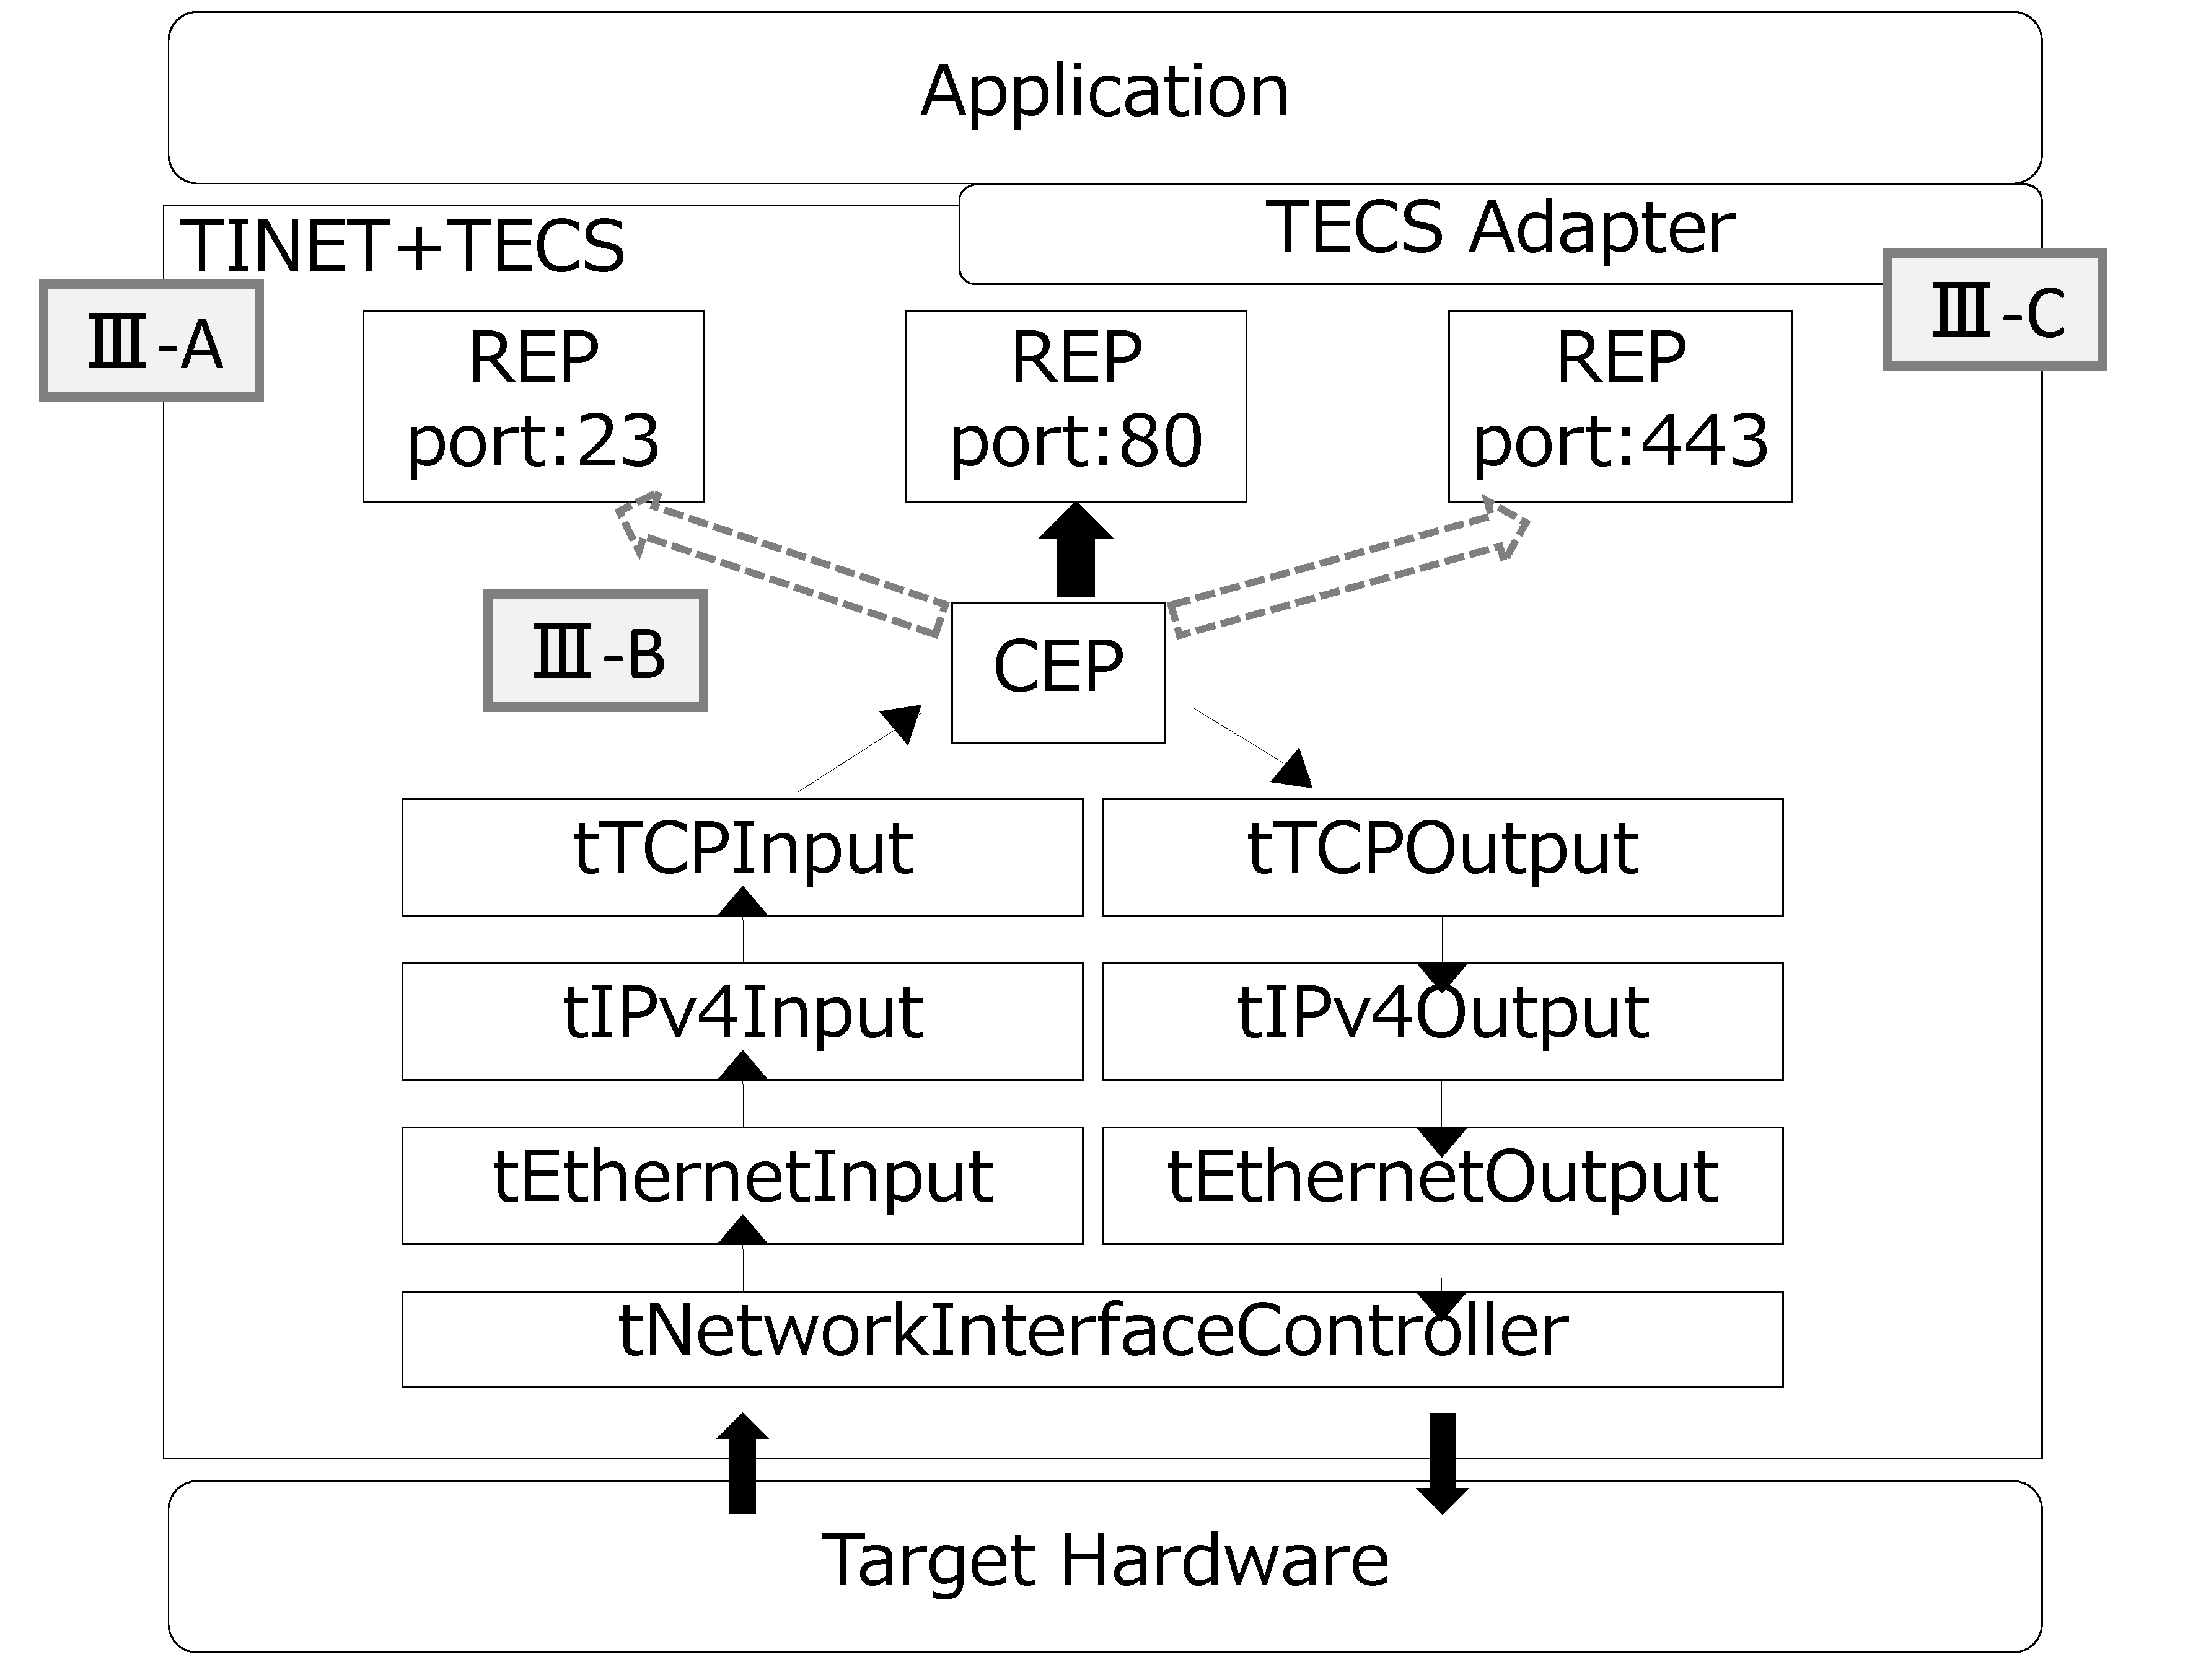
\includegraphics[width=8.0cm,clip]{figure/SystemModel.pdf}
    \caption{System model of TINET+TECS}
    \label{fig:SystemModel}
\end{figure}

\subsection{TINET}
\label{sec:TINET}

TINET is a compact TCP/IP protocol stack for embedded systems based on the ITRON\footnote{ITRON is a realtime operating system (RTOS) developed by the TRON project.} TCP/IP API Specification \cite{url:ITRON_TCP/IP_API_Spec}, developed by the TOPPERS Project \cite{url:TOPPERS}.
TINET has been released as an open-source tool.

To satisfy restrictions for embedded systems in terms of, for example, memory capacity, size, and power consumption, TINET supports the following functions:

\begin{itemize}
    \item minimum copy frequency,
    \item elimination of dynamic memory control,
    \item asynchronous interfacing,
    \item error detailing per API.
\end{itemize}

\subsubsection{Overview}

TINET runs as middleware on TOPPERS/ASP3 \cite{par:ASP3} \cite{url:ASP3}, a real-time kernel based on $\mu$ITRON \cite{par:microITRON}.
As it is compatible with TOPPERS RTOS, TINET also supports other RTOSs such as TOPPERS/ASP and TOPPERS/JSP.

Fig. \ref{fig:TINETHierarchyDiagram} shows the hierarchy diagram of TINET and TOPPERS/ASP3.
% TINET supports ITRON TCP/IP API such as {\it tcp\_snd\_buf}, {\it tcp\_rcv\_buf}, {\it udp\_snd\_buf}, and {\it udp\_rcv\_buf}.
Users transmit and receive data using a Communication End Point (CEP), an interface that functions like a socket.
In the transmission process, headers are attached to the data body passed to the CEP at each protocol layer before the data are transmitted from the network device.
In the reception process, the headers of the data bodies received by the network device are analyzed at each protocol layer, and the data are then passed to the CEP.

A TCP reception point called the REP stands by to receive connection requests from the partner side.
The REP has an IP address ({\it myaddr}) and a port number ({\it myportno}) as attributes and performs functions such {\it bind()} and {\it listen()}.

In TINET, the amount of data copying between each protocol layers is minimized.
In standard computing systems, the TCP/IP protocol stack has large overheads in terms of execution time and memory consumption because the data are copied at each protocol layer.
To solve this problem, TINET does passes the pointer of the data buffer between each protocol layer instead of performing data copying.

\begin{figure}[t]
    \centering
    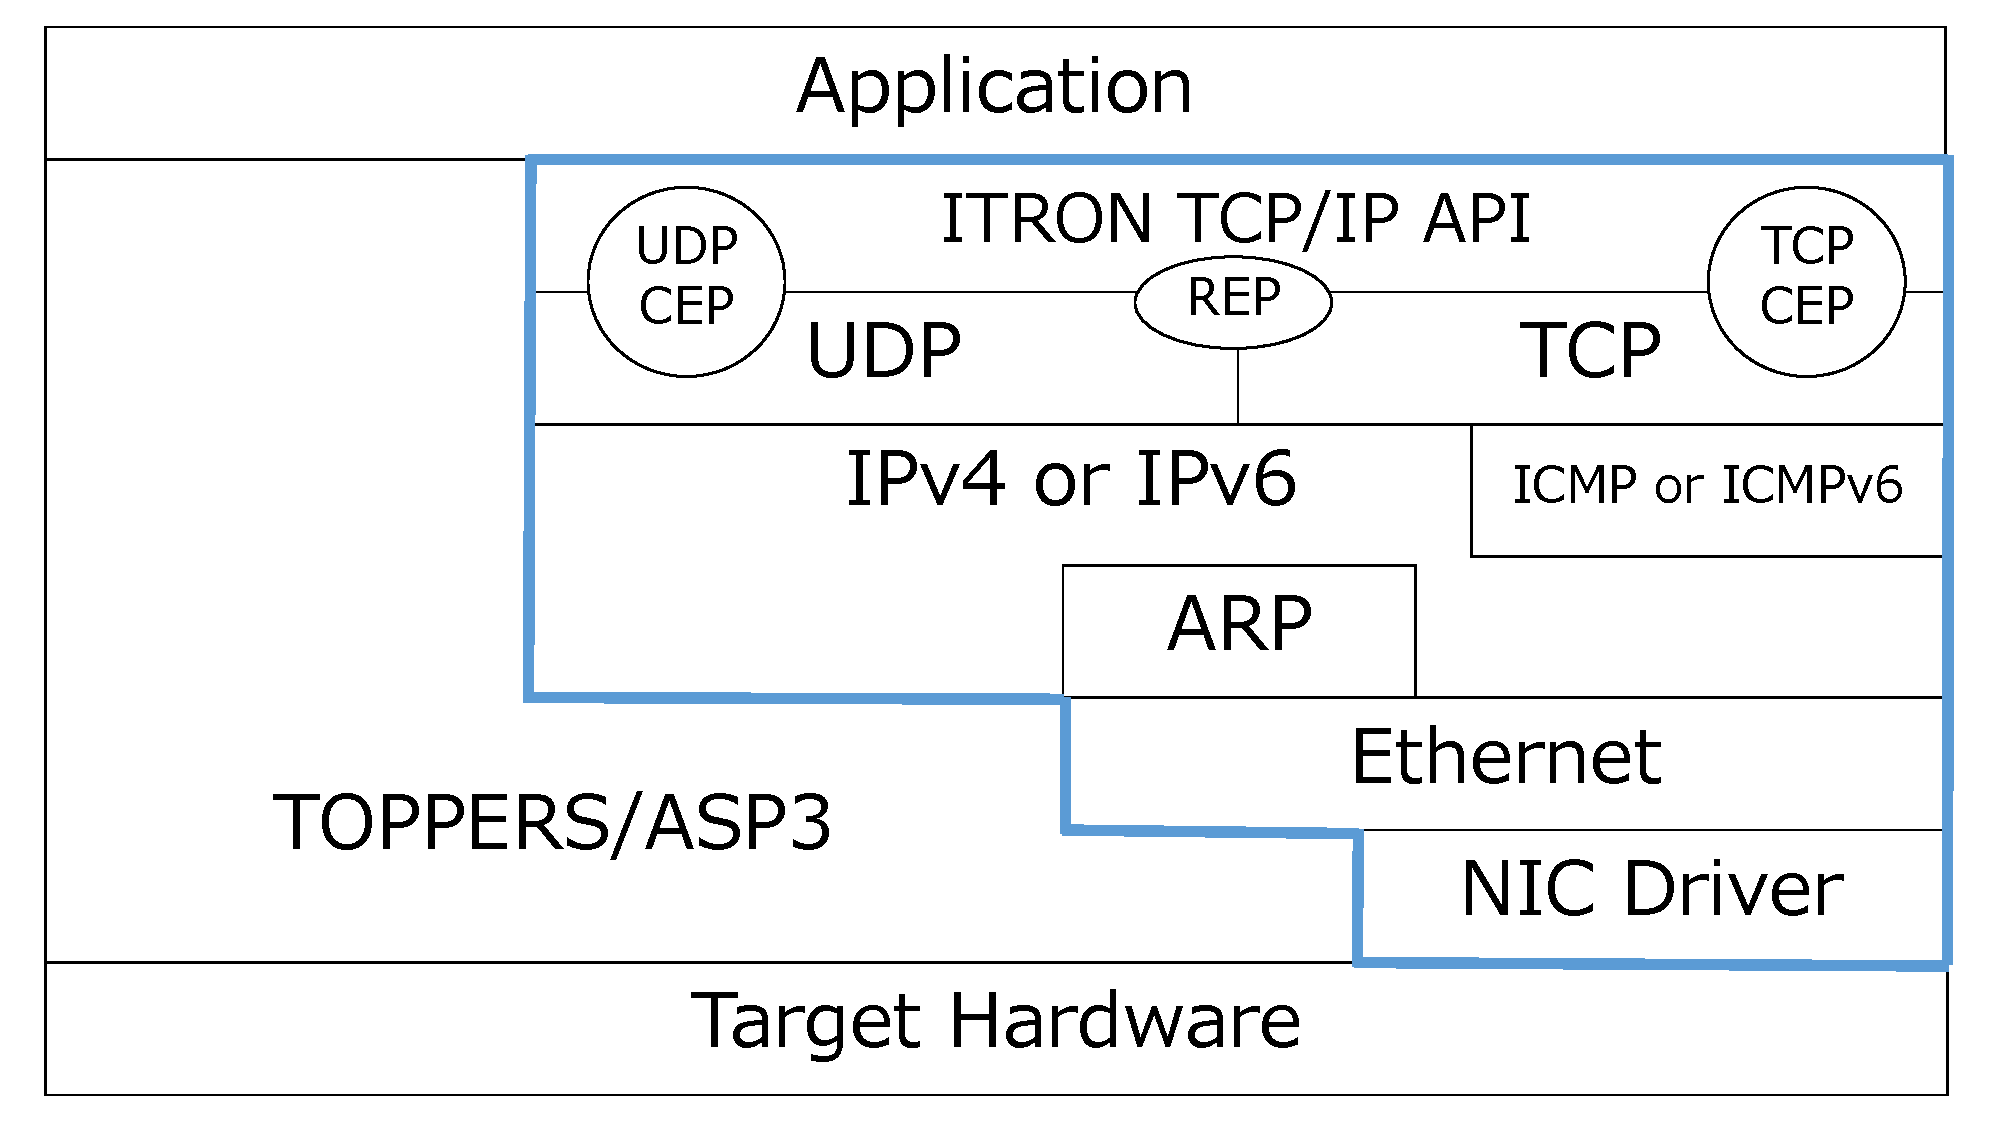
\includegraphics[width=8.0cm,clip]{figure/TINETHierarchyDiagram.pdf}
    \caption{TINET and TOPPERS/ASP3 hierarchy diagrams}
    \label{fig:TINETHierarchyDiagram}
\end{figure}

\subsection{TECS}
\label{sec:TECS}

TECS is a component system suitable for embedded systems that can increase productivity and reduce development costs based on the improved reusability of software components.
TECS also provides component diagrams that can help developers visualize the overall structure of a system.

In TECS, component deployment and composition are performed statically, and as a consequently, component connection does not incur significant overhead, and memory requirements can be reduced.
TECS has various features such as source level portability and fine-grained components and can be implemented in C.

\begin{figure}[t]
    \centering
    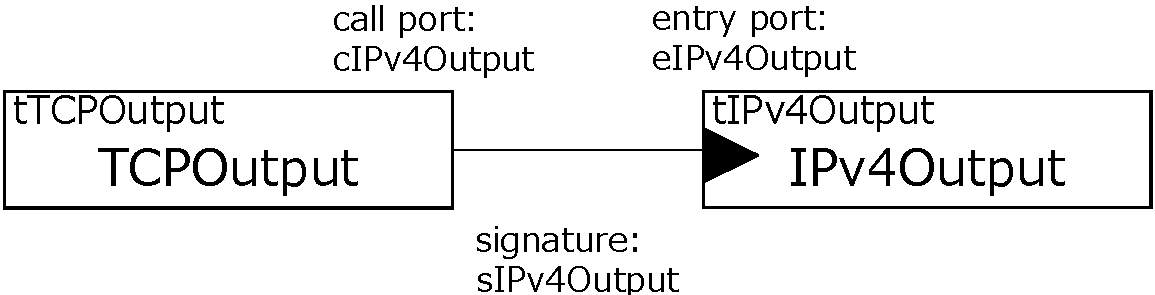
\includegraphics[width=8.0cm,clip]{figure/ComponentDiagram.pdf}
    \caption{Component diagram}
    \label{fig:ComponentDiagram}
\end{figure}

\subsubsection{Component model}

Fig. \ref{fig:ComponentDiagram} shows a component diagram.
{\it Cells}, which are instance of components in TECS, consist of {\it entry} ports, {\it call} ports, attributes, and internal variables.
An {\it entry} port is an interface that provides functions to other {\it cells}, whereas a {\it call} port is an interface that enables the use of other {\it cells}' functions.
Each {\it cell} has one or more {\it entry} ports and {\it call} ports.
{\it Cell} functions are implemented in C.

The type of {\it entry}/{\it call} port is defined by a {\it signature}, which is a set of functions that defines the interface definition of the {\it cell}.
The {\it cell's} {\it call} port can be connected to the {\it entry} port of another {\it cell} by the same {\it signature}.
Note that {\it celltype} defines one or more {\it call}/{\it entry} ports, attributes, and internal variables of a {\it cell}.

\subsubsection{Component description}

In TECS, components are described using component description language (CDL).
CDL can be divided into three categories: {\it signature}, {\it celltype}, and build description.
These components are described as follows.

\begin{description}
    \item[{\bf Signature Description}]\mbox{}\\
        The {\it signature} defines a {\it cell} interface.
        The {\it signature} name follows the keyword {\it signature} and takes the prefix ``s''--for instance, sIPv4Output (Fig. \ref{src:signature}).
        To clarify the function of an interface, specifiers such as [in], [out], and [inout] are used in TECS to represent the input, output, and input/output, respectively.
        Similarly, [size\_is({\it len})] represents an array of size {\it len}.
\begin{figure}[t]
\centering
\begin{lstlisting}
signature sIPv4Output {
  T_IN4_ADDR getIPv4Address(void);
  ER         getOffset([inout]T_OFF_BUF *offset);
  ER         setHeader([inout,size_is(size)]
                        int8_t *outputp,
                        [in]int32_t size,
                        [in]T_IN4_ADDR dstaddr,
                        [in]T_IN4_ADDR srcaddr);
    /* Omit: other functions */
};
\end{lstlisting}
\caption{Signature description}
\label{src:signature}
\end{figure}
    \item[{\bf Celltype Description}]\mbox{}\\
        The {\it celltype} defines the {\it entry} ports, {\it call} ports, attributes, and variables.
        A {\it celltype} name with the prefix ``t'' follows the keyword {\it celltype}, e.g., tIPv4Output (Fig. \ref{src:celltype}).
        To define {\it entry} ports, a {\it signature}, e.g., sIPv4Output, and an {\it entry} port name, e.g., eIPv4Output, follow the keyword {\it entry}.
        {\it Call} ports are defined similarly.
        Attributes and variables follow the keywords {\it attr} and {\it var}, respectively.
\begin{figure}[t]
\centering
\begin{lstlisting}
celltype tIPv4Output {
    /* Entry port */
    entry sIPv4Output eOutput;

    /* Call port */
    call sEthernetOutput cEthernetOutput;
    /* Omit: other call ports */

    attr {  /* Attribute */
        uint16_t fragInit = 0;
    };
    var {   /* Variable */
        uint16_t fragId = fragInit;
    };
};
\end{lstlisting}
\caption{Celltype description}
\label{src:celltype}
\end{figure}
    \item[{\bf Build Description}]\mbox{}\\
        The build description is used to instantiate and connect {\it cell}s.
        Fig. \ref{src:build} shows an example of a build description.
        A {\it celltype} name and {\it cell} name, e.g., tIPv4Output and IPv4Output, respectively, follow the keyword {\it cell}.
        A {\it call} port, {\it cell}'s name, and an {\it entry} port are described in that order to compose {\it cell}s,
        In Fig. \ref{src:build}, {\it entry} port eIPv4Output in {\it cell} IPv4Output is connected to {\it call} port cIPv4Output in {\it cell} TCPOutput.
        {\it C\_EXP} can be used to call macros defined in C files.

\begin{figure}[t]
\centering
\begin{lstlisting}
cell tIPv4Output IPv4Output {
    /* Omit: other build description */
    
    fragInit = 0; /* Attribute */
};
cell tTCPOutput TCPOutput {
    cIPv4Output = IPv4Output.eOutput;
    /* Omit: other build description */
};
\end{lstlisting}
\caption{Build description}
\label{src:build}
\end{figure}

\end{description}

\section{Design and Implementation}
\label{sec:Design and Implementation}

This section describes design and implementation of the proposed framework, TINET+TECS.
The proposed framework is component-based TCP/IP protocol stack for embedded systems, i.e., componentized TINET using TECS.
In addition, A TECS novel functionality, dynamic connection method, and TECS adapter to support legacy codes are described with the use case of the proposed framework.

\subsection{TINET+TECS}
TINET+TECS, the proposed componentized TCP/IP protocol stack, consists of some TECS components.
This section describes the components of TINET+TECS framework with component diagrams.
% In addition, TECS functionalities applied to the proposed system such as {\it send}/{\it receive} specifier and adapter are explained.

\subsubsection{Components of protocol stack}

The components of a protocol stack for TINET+TECS is shown in Fig. \ref{fig:ComponentProtocolStack}.
Note that some small particle components such as a kernel object, dataqueques, and semaphores are omitted to simplify the component diagram.
In TINET+TECS, the components are divided for each protocol, and the functionalities such as input function and output function are defined as each a component.
Therefore, software visibility is improving because of small grain components.

\begin{figure}[t]
    \centering
    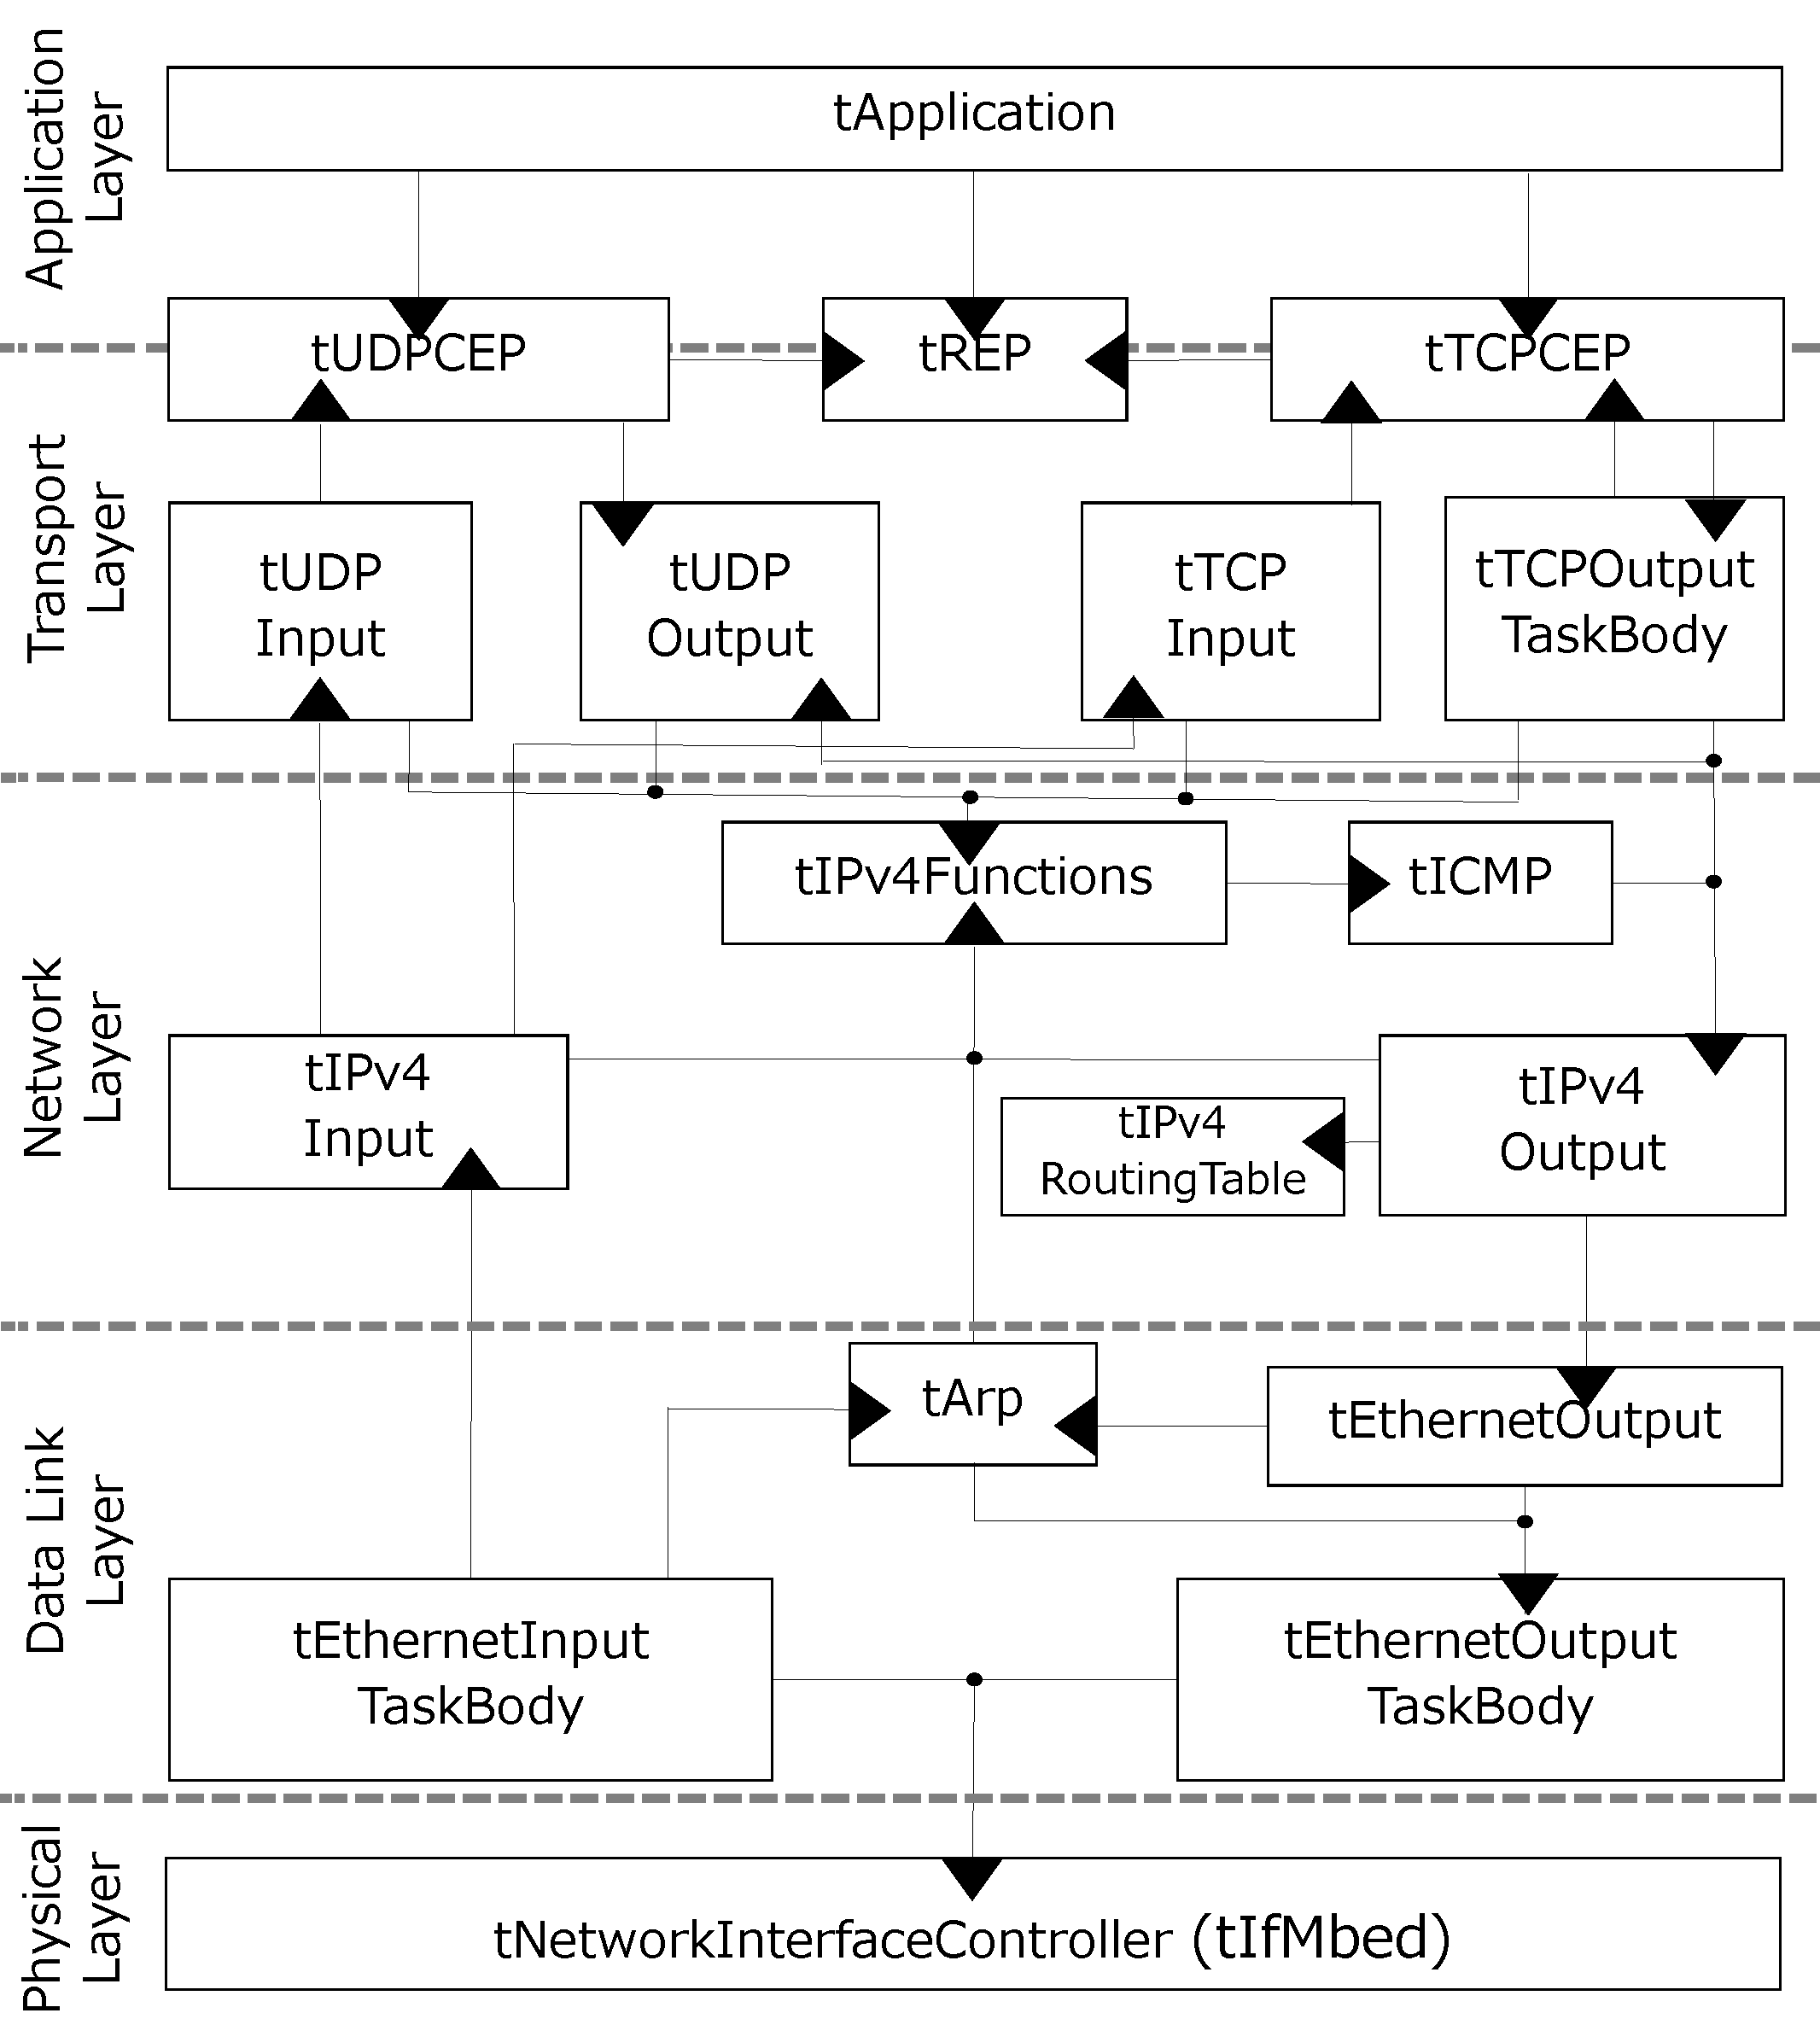
\includegraphics[width=8.0cm,clip]{figure/ComponentProtocolStack.pdf}
    \caption{Component diagram of protocol stack}
    \label{fig:ComponentProtocolStack}
\end{figure}

The components of each protocol are described below.\\

{\bf Application layer:}
An application in TINET+TECS is implemented as a component such as tApplication.
Software with TINET uses ITRON TCP/IP API \cite{url:ITRON_TCP/IP_API_Spec} such as {\it tcp\_snd\_dat} and {\it tcp\_rcv\_dat}.
In TINET+TECS, the application component calls TECS functions such as {\it cTCPAPI\_sendData} and {\it cTCPAPI\_receiveData}.
Moreover, TINET+TECS supporting a TECS adapter (\ref{sec:TECS Adapter}), an existing application with TINET can run on TINET+TECS framework without transporting.
Therefore, software can be developed either with existing methods or as a TECS component.

{\bf Transport layer:}
tTCPCEP (tUDPCEP) is a CEP component for TCP (UDP), and tREP is a REP component.
For example, a server program supporting multiple clients can be developed by preparing the multiple tTCPCEP components.
tTCPInput (tUDPInput) and tTCPOutput (tUDPOutput) are components performing the receiving and sending processing respectively in the transport layer.

{\bf Network layer:}
tIPv4Input and tIPv4Output are components performing the receiving and sending processing respectively in the network layer.
tIPv4Functions component performs some functions such as checksum, tICMP component is for the ICMP protocol, and tIPv4RoutingTable component operates a routing table.

{\bf Data link layer:}
tEthernetInputTaskBody and tEthernetOutputTaskBody (tEthernetOutput) are components performing the receiving and sending processing respectively in the data link layer.
tArp component is for the ARP protocol.

{\bf Physical layer:}
tNetworkInterfaceContoroller component implements a network device driver.
Software can run on other devices by replacing the component because only the component depends on the target device.\\

To utilize the protocol stack as same as the original TINET, communication object components such as tTCPCEP, tUDPCEP, and tREP are defined as an interface between TINET+TECS and an application.
The communication object component is a component corresponding to a CEP or REP of the original TINET.
Application developers can utilize the TINET+TECS functionalities by generating and combining as many components as necessary.

The protocol stack of TINET+TECS supports coexistence of multiple protocols.
By developing the IPv6 and Point-to-Point Protocol (PPP) components, TINET+TECS can make IPv4 and IPv6 coexist and support PPP without a modification of component implementation.

\subsubsection{Memory allocator component} 

The original TINET eliminates dynamic memory control to meet the severe memory restriction of embedded systems.
A memory area for sending/receiving data in the protocol stack is allocated and released within a predetermined area.
Memory allocator component performs the elimination of dynamic memory control in TINET+TECS.
The component provides a requested memory area from the memory area statically allocated.

The memory allocator component connects to as many tFixedSizeMemoryPool as needed, shown in Fig. \ref{fig:tMemoryAllocator}.
tFixedSizeMemoryPool is a componentized kernel object of TOPPERS/ASP3 to alloc and release a memory area of the requested size. 
tFixedSizeMemoryPool components with various sizes are prepared, and an appropriate memory area can be allocated according to the used data size.
On the other hands, all components which need allocate and deallocate memory connect to the memory allocator component, e.g., tTCPInput and tEthernetOutput.

In addition, TINET+TECS utilizes {\it send/receive} specifier of TECS to minimize the memory copy frequency, which is a functionality supported by TINET.

\begin{figure}[t]
    \centering
    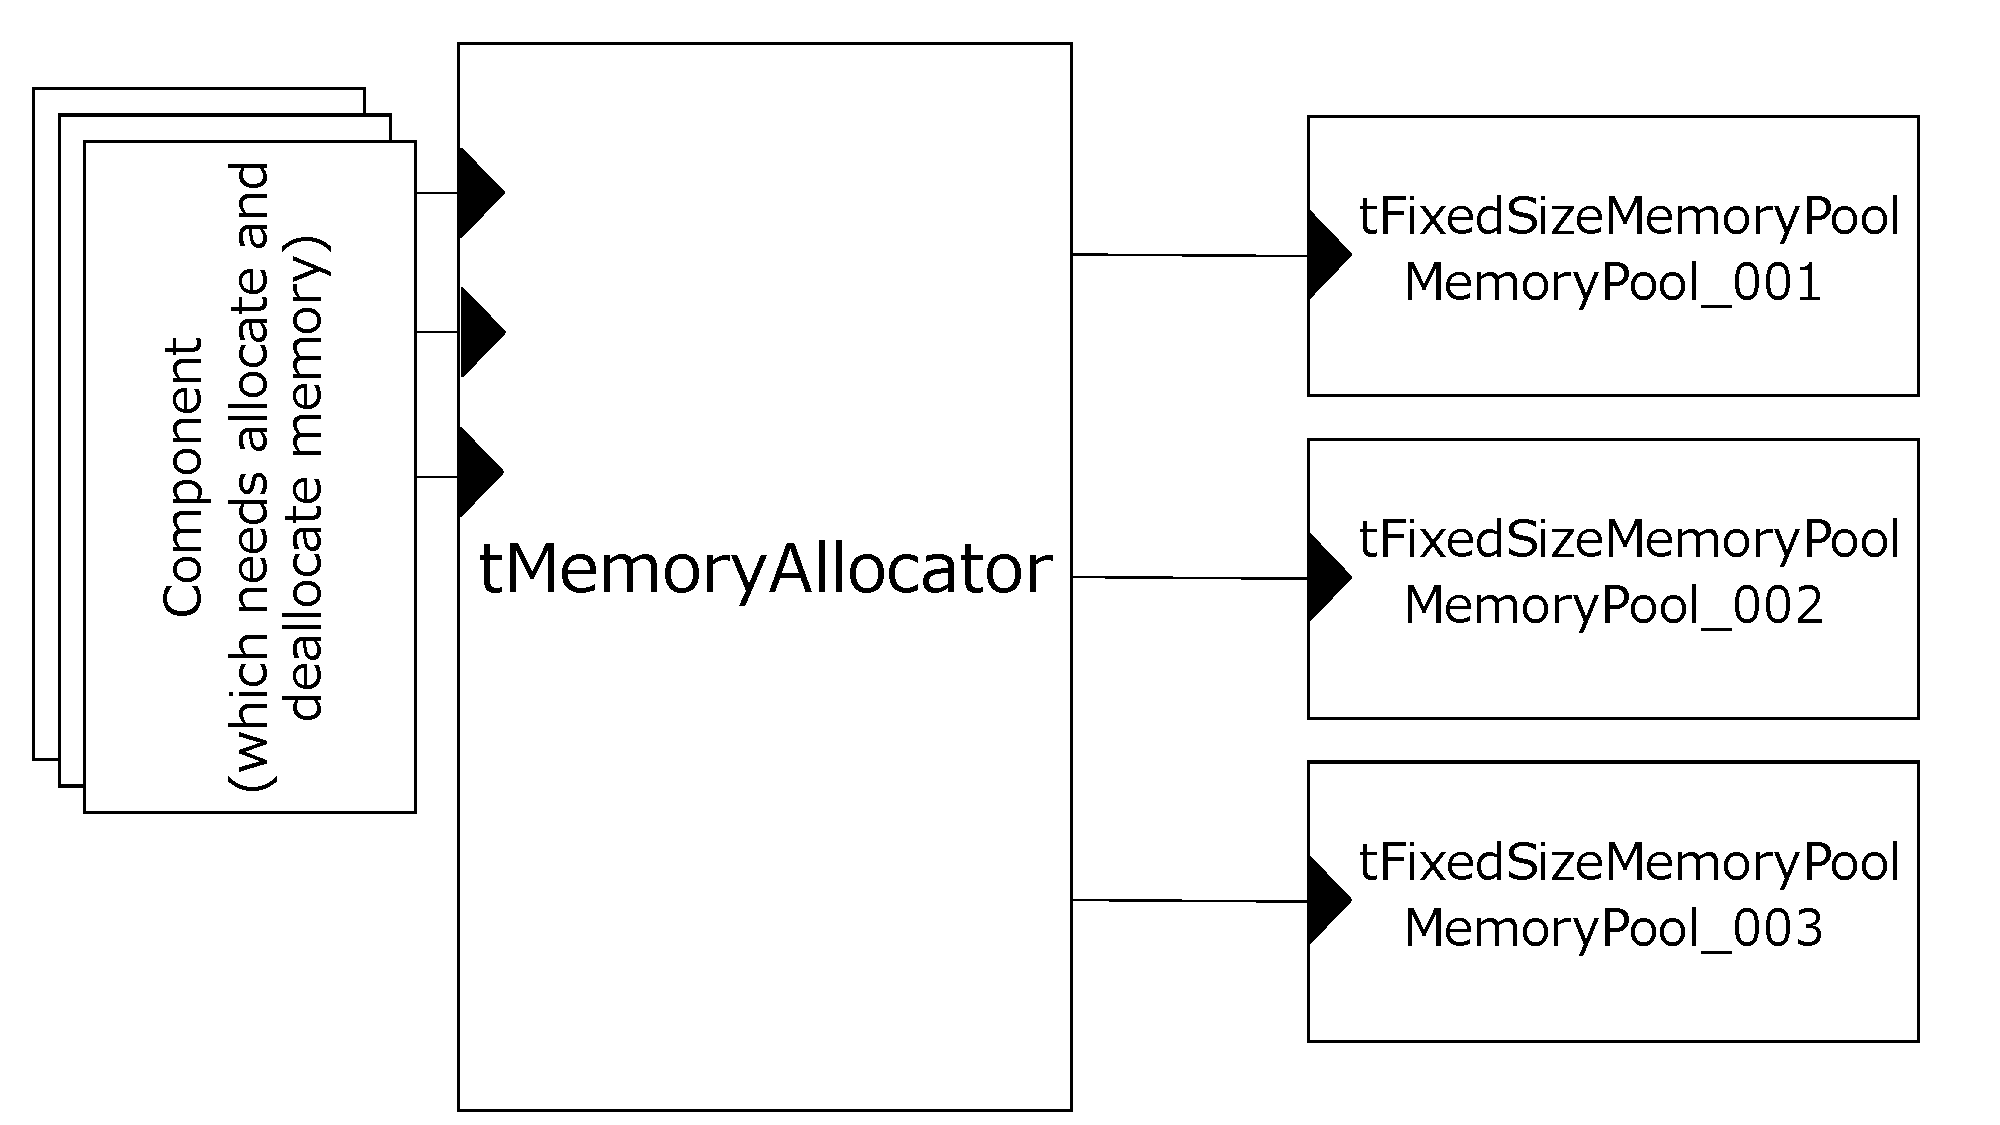
\includegraphics[width=8.0cm,clip]{figure/tMemoryAllocator.pdf}
    \caption{Component diagram of tMemoryAllocator}
    \label{fig:tMemoryAllocator}
\end{figure}

\begin{figure}[t]
    \centering
    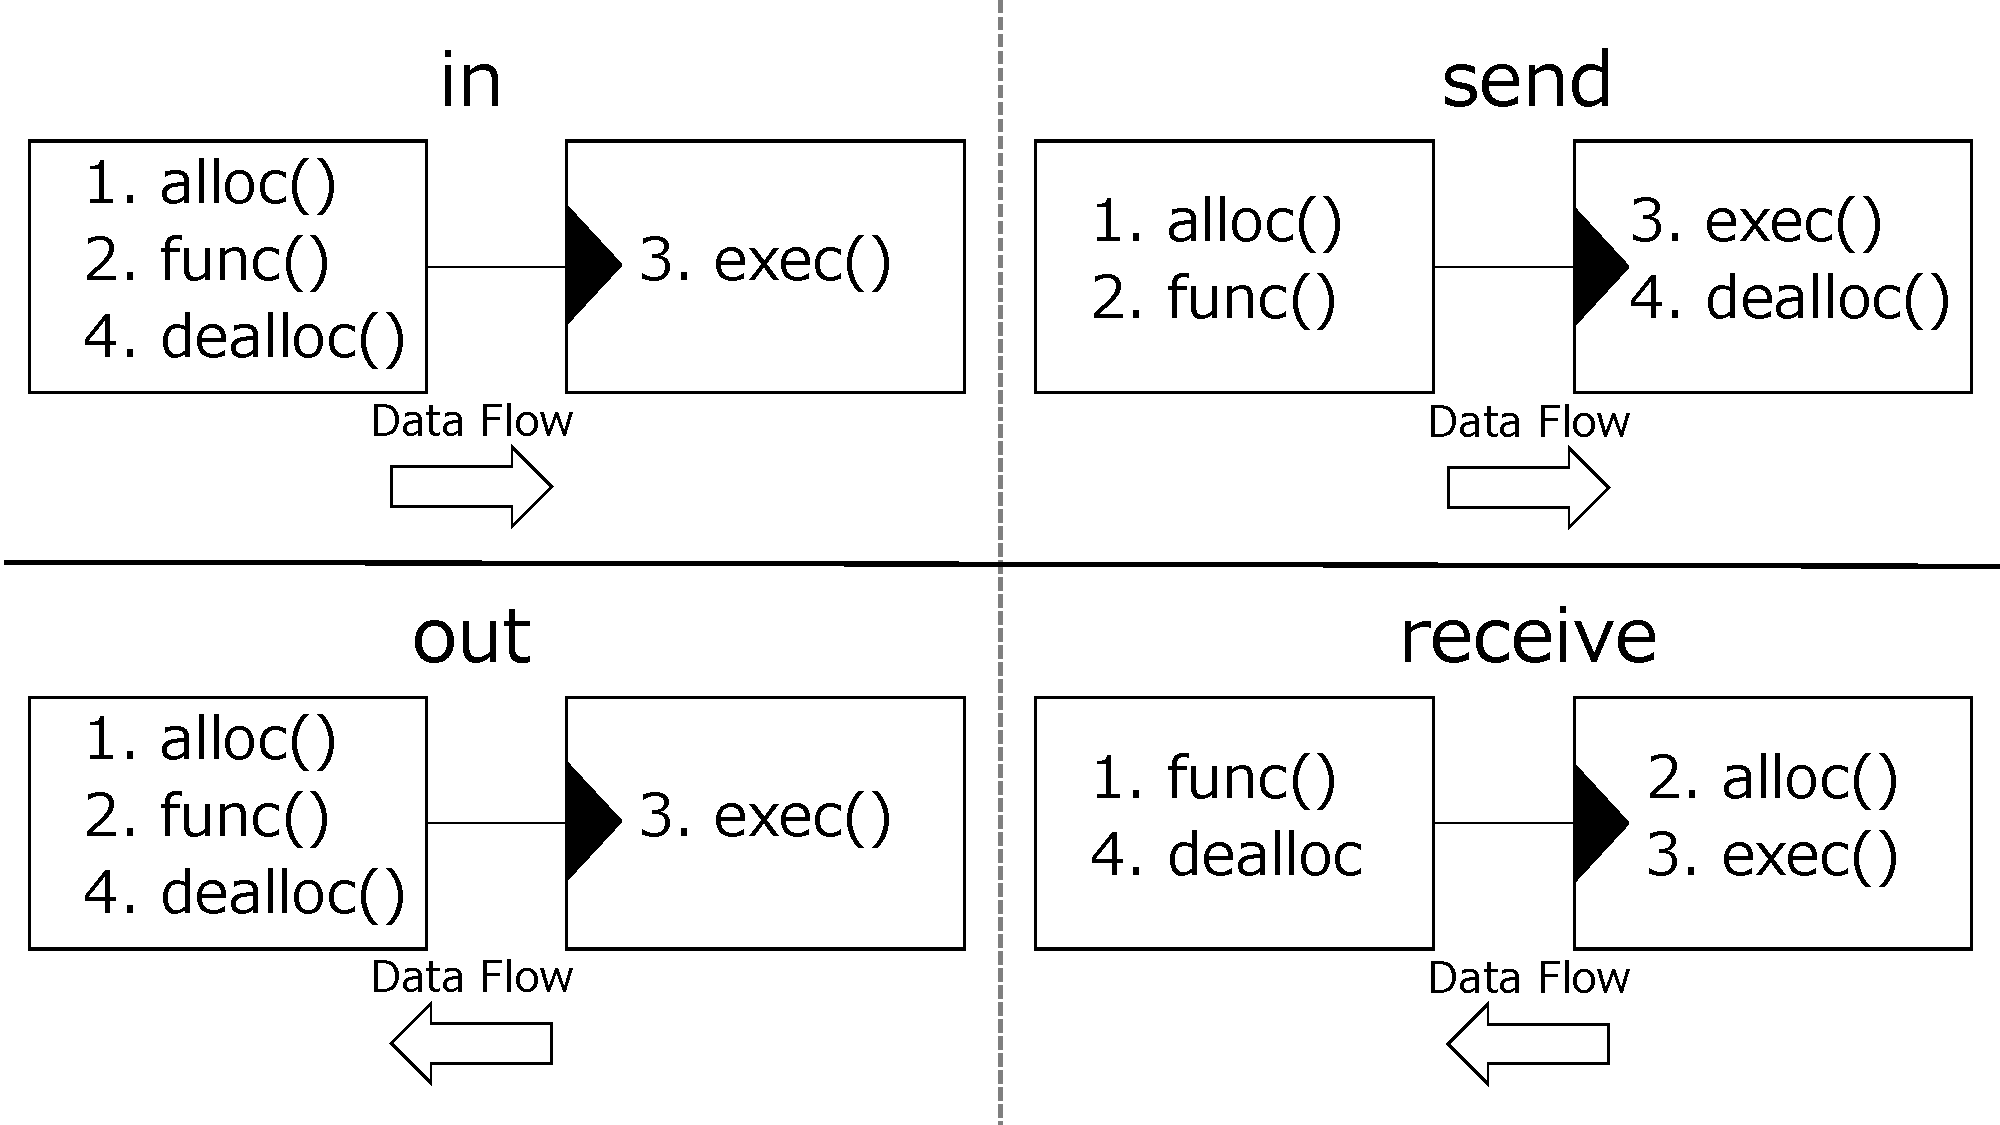
\includegraphics[width=8.0cm,clip]{figure/SendReceive.pdf}
    \caption{Differences between in/out and send/receive}
    \label{fig:SendReceive}
\end{figure}

{\bf send/receive specifier:}
TECS supports {\it send}/{\it receive} specifiers, which are interface specifiers \cite{par:RPC}.
TINET+TECS uses {\it send} and {\it receive} specifiers instead of {\it in} and {\it out} to reduce the number of copies.

{\it in} is a specifier for input arguments.
A callee side uses the memory of arguments with {\it in} during executing the callee function.
When the processing returns to the caller side, the caller can reuse and deallocate the memory.

{\it send} is also a specifier for transferring data to a callee from a caller such as {\it in}.
The difference between {\it in} and {\it send} is whether to deallocate the data memory in a caller or callee, shown in Fig. \ref{fig:SendReceive}.
In case of {\it in} specifier, both allocating and deallocating the data memory are performed in the caller.
On the other hand, in case of {\it send}, the caller allocates the data memory and the callee deallocates it.

{\it out} is a specifier for output arguments.
A callee writes data in the memory allocated by a caller, and the caller receives the data.

{\it receive} is also a specifier for a caller receiving data from a callee such as {\it out}.
The difference between {\it out} and {\it receive} is whether to allocate the data memory in a caller or callee, shown in Fig. \ref{fig:SendReceive}.
While, in case of {\it out}, a callee writes data in the memory allocated by a caller, in case of {\it receive}, the callee allocates the data memory.
Deallocating the memory is performed in the caller in both cases.

As shown in Fig. \ref{src:SendReceive}, the arguments of sending and receiving data such as {\it outputp} and {\it inputp} are defines with the {\it send/receive} specifiers in the signature description.

\begin{figure}[t]
\centering
\begin{lstlisting}
signature sNicDriver {
  void start(
    [send(sNetworkAlloc),size_is(size)]
        int8_t *outputp,
    [in]int32_t size,
    [in]uint8_t align);
  void read(
    [receive(sNetworkAlloc),size_is(*size)]
        int8_t **inputp,
    [out]int32_t *size,
    [in]uint8_t align);
    /* Omit: other functions */
};
\end{lstlisting}
\caption{Signature description of the nic driver (An example of send/receive)}
\label{src:SendReceive}
\end{figure}

% \subsubsection{Network timer component}


\subsection{Dynamic Connection of TECS}
\label{sec:DynamicConnection}

\begin{figure}[t]
    \centering
    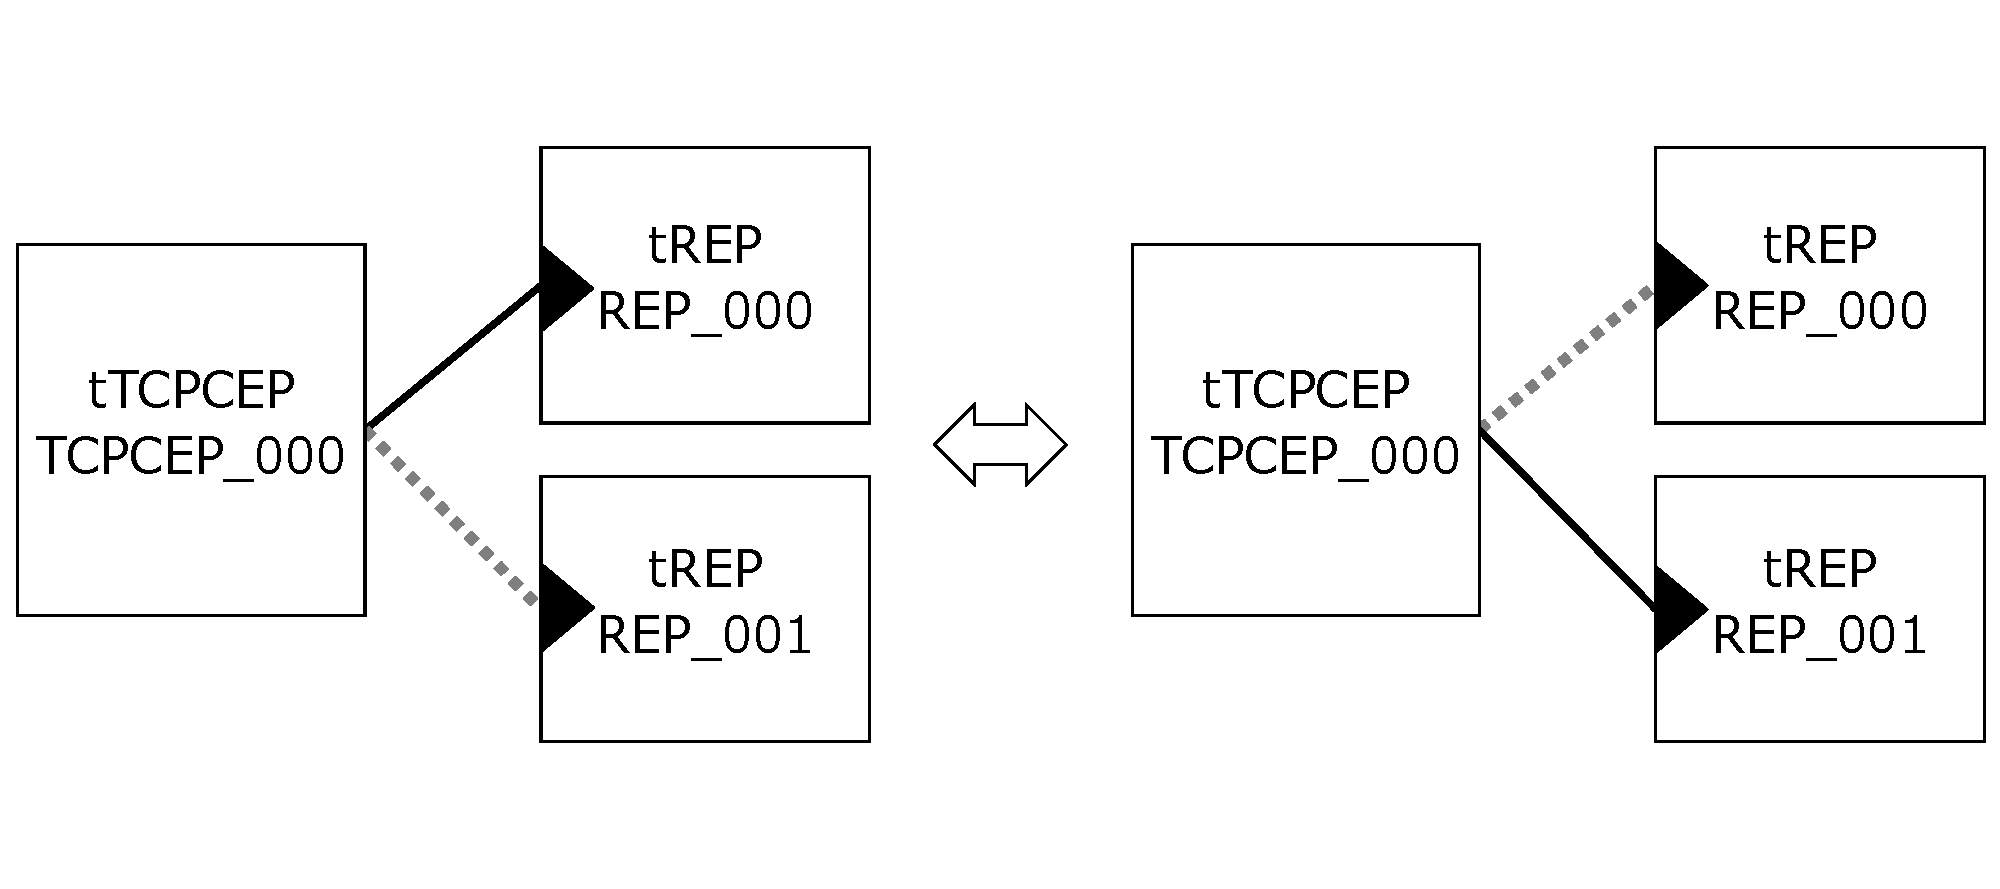
\includegraphics[width=8.0cm,clip]{figure/DynamicConnection.pdf}
    \caption{Dynamic connection}
    \label{fig:DynamicConnection}
\end{figure}

TECS supports dynamic connection as a new functionality.
Dynamic connection is a method to switch the binding of components at runtime as shown in Fig. \ref{fig:DynamicConnection}.
Note that all components are statically generated in TECS.
TECS can optimize the overhead of componentization because components are statically configured.
Dynamically generating the components causes a lot of memory consumption, which is a serious problem for embedded systems with strict memory constraint.
The proposed framework realizes the componentization of TINET while satisfying the memory constraint, because components statically generate and dynamically connect in TECS.

TINET+TECS utilizes the dynamic connection to switch between CEP and REP components as shown in Fig. \ref{fig:DynamicConnectionUseCase}.
In a server application, CEP is associated with REP in the state waiting for connection request from clients\footnote{ITRON TCP/IP API Specification \cite{url:ITRON_TCP/IP_API_Spec}\\tcp\_acp\_cep(ID cepid, ID repid, T\_IPV4EP *p\_dstaddr, TMO tmout)}.
For example, when processing with HTTP protocol, CEP passively opens with REP of port number 80.

\begin{figure}[t]
    \centering
    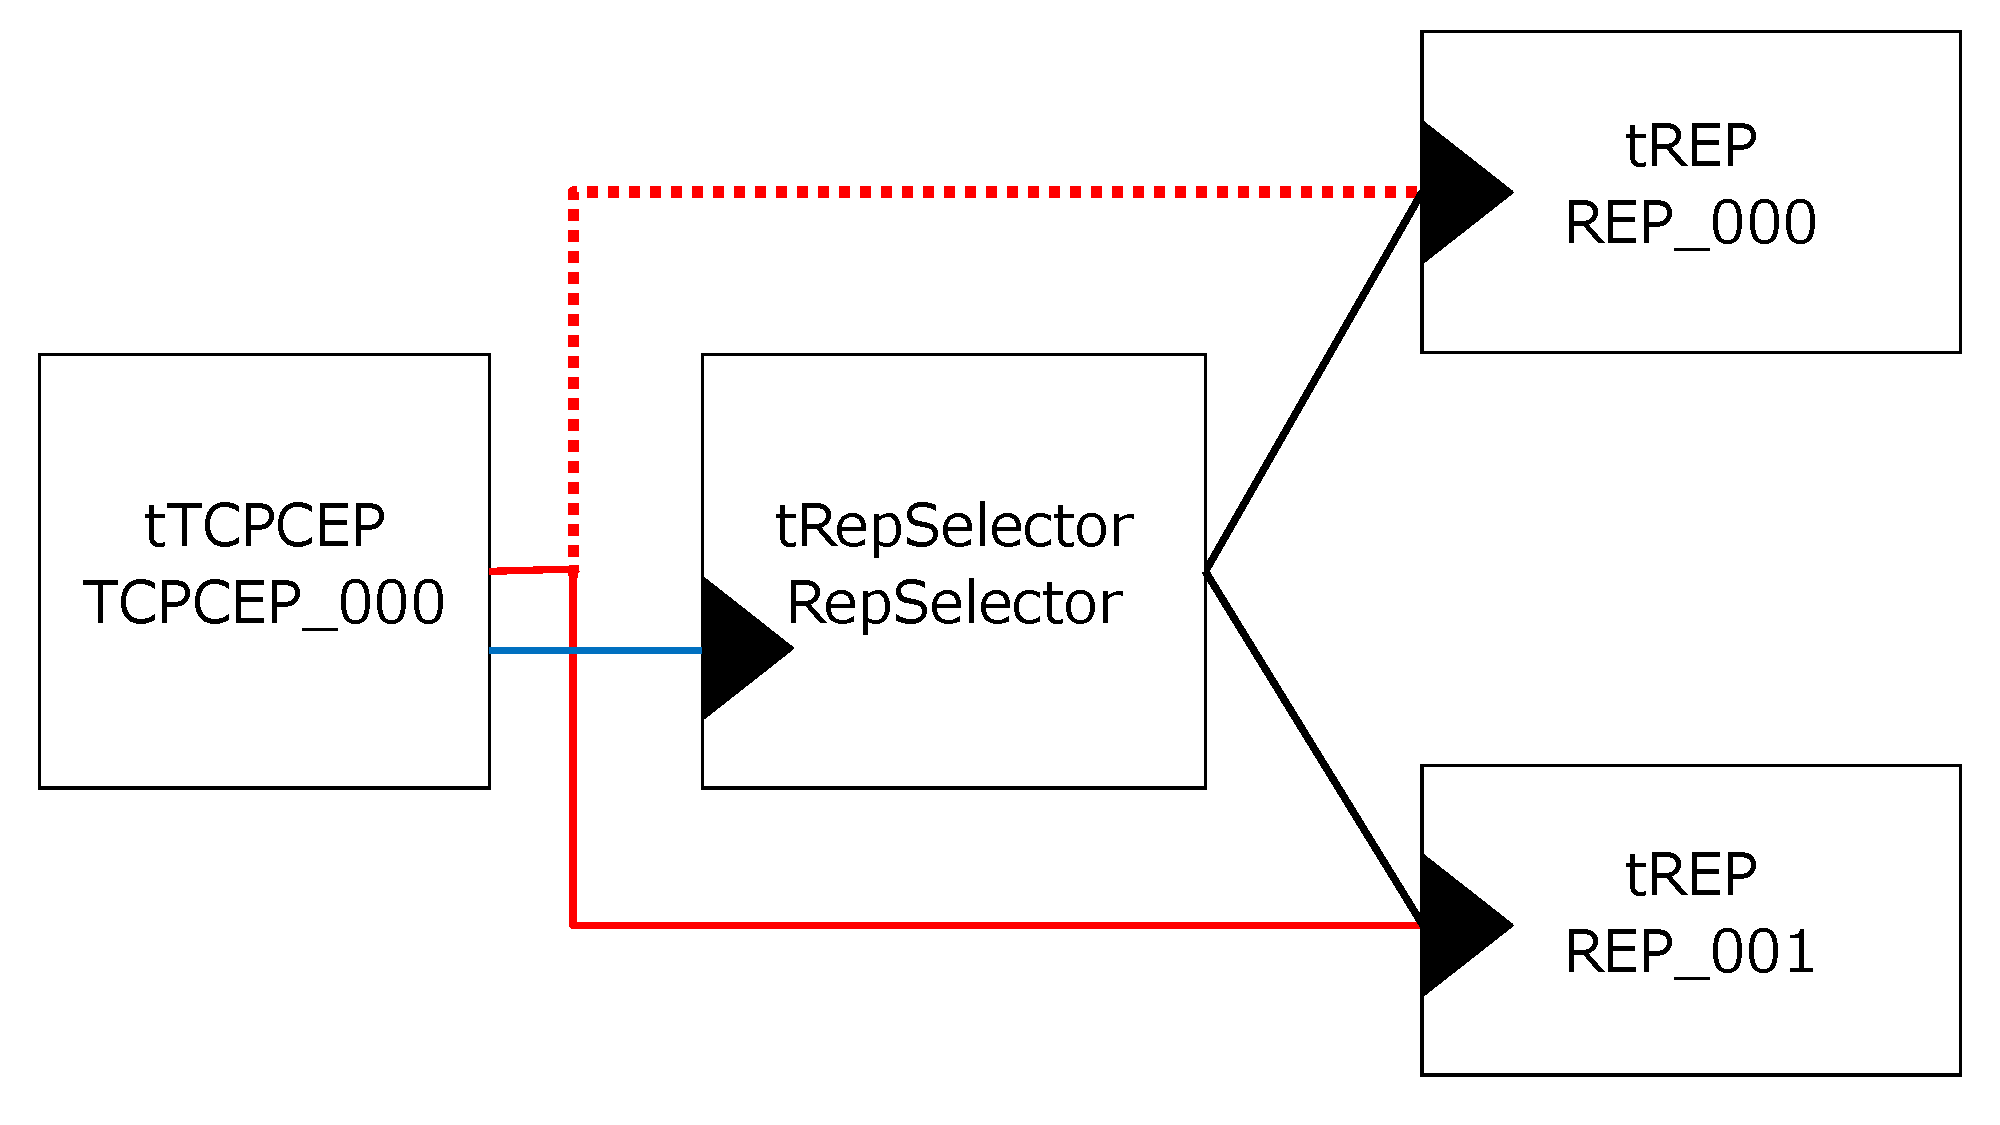
\includegraphics[width=8.0cm,clip]{figure/DynamicConnectionUseCase.pdf}
    \caption{Dynamic connection between CEP and REP}
    \label{fig:DynamicConnectionUseCase}
\end{figure}

To utilize dynamic connection, the selector should be defined.
The selector connects all the components that can be dynamically connnected, to refer the descriptor of them.
Descriptor is an identifier to access the component \cite{par:optimization}.
cREP ports are call ports array, which connect the number of tREP cells (Line 9 in Fig. \ref{src:DynamicCDLcode}).
{\it [ref\_desc]} is described to identify the call port refers to descriptors. 
In the case of Fig. \ref{fig:DynamicConnectionUseCase}, the tRepSelector cell connects all tREP cells.

A CEP component has two call ports.
cRepSelector port connects eRepSelector port of tRepSelector cell and cREP4 port connects either of tREP cells (Lines 13-15 in Fig. \ref{src:DynamicCDLcode}).
cREP port is defined with {\it [dynamic]} to identify the call port dynamically switch the components.
The call port with {\it [dynamic]} specifier is not optimized and allocated in RAM by a plug-in.

\begin{figure}[t]
\centering
\begin{lstlisting}
signature sRepSelector {
    void  getRep([out]Descriptor(sREP4) *desc,
                 [in]int_t i);
};

celltype tRepSelector {
    entry sRepSelector eRepSelector;
    [ref_desc]
        call sREP4 cREP[NUM_REP];
};

celltype tTCPCEP {
    call sRepSelector cRepSelector;
    [dynamic]
        call sREP4 cREP;
    /* Omit: other call/entry ports */
    /* Omit: attributes and variables */
};
\end{lstlisting}
\caption{Signature and celltype description for dynamic connection}
\label{src:DynamicCDLcode}
\end{figure}

Fig. \ref{src:DynamicCcode} shows a sample code of dynamic connection.
The eAPI\_accept function is the function wrapping {\it tcp\_acp\_cep} with TECS, which is utilized to be the state waiting for connection request.
In the function, dynamic connection is performed as shown in Fig. \ref{src:DynamicCcode}.
First, get the descriptor of REP to be joined (Line 3 in Fig. \ref{src:DynamicCcode}).
The first argument, {\it \&desc}, is a variable to store the descriptor information, and the second argument, {\it repid}, is the index of tREP cells.
Next, set the desctriptor (Line 5 in Fig. \ref{src:DynamicCcode}).
cREP port combines the tREP cell that descriptor specify.
Thus, the tCEP cell can call the function of tREP cell to be joined (Line 7 in Fig. \ref{src:DynamicCcode}).

\begin{figure}[t]
\centering
\begin{lstlisting}
eAPI_accept (.., ..) {
    /* Get a descriptor of intended REP cell */
    cRepSelector_getRep(&desc, repid);
    /* Set the descriptor */
    cREP_set_descriptor(desc);
    /* Call the function of intended REP cell */
    cREP_getEndpoint();
}
\end{lstlisting}
\caption{Accept function (a dynamic connection example)}
\label{src:DynamicCcode}
\end{figure}

\subsection{TECS Adapter}
\label{sec:TECS Adapter}

TECS supports {\it Adapter} functionality which enables to call a function in TECS from existing C codes.
An adapter is implemented between C codes and a TECS component, and links a C function to a TECS function shown in Fig. \ref{fig:TECS_Adapter}.
In TINET+TECS, when the application calls an API such as {\it tcp\_snd\_dat}, the adapter component calls the function of tTCPCEP such as {\it eAPI\_sendData}.
Note that {\it tcp\_snd\_dat} is defined with the name {\it eAPI\_sendData} in TINET+TECS.
The adapter wraps the APIs used in the existing applications into TECS functions.
Therefore, software developers can utilize an existing TCP/IP application by using the adapter.

\begin{figure}[t]
    \centering
    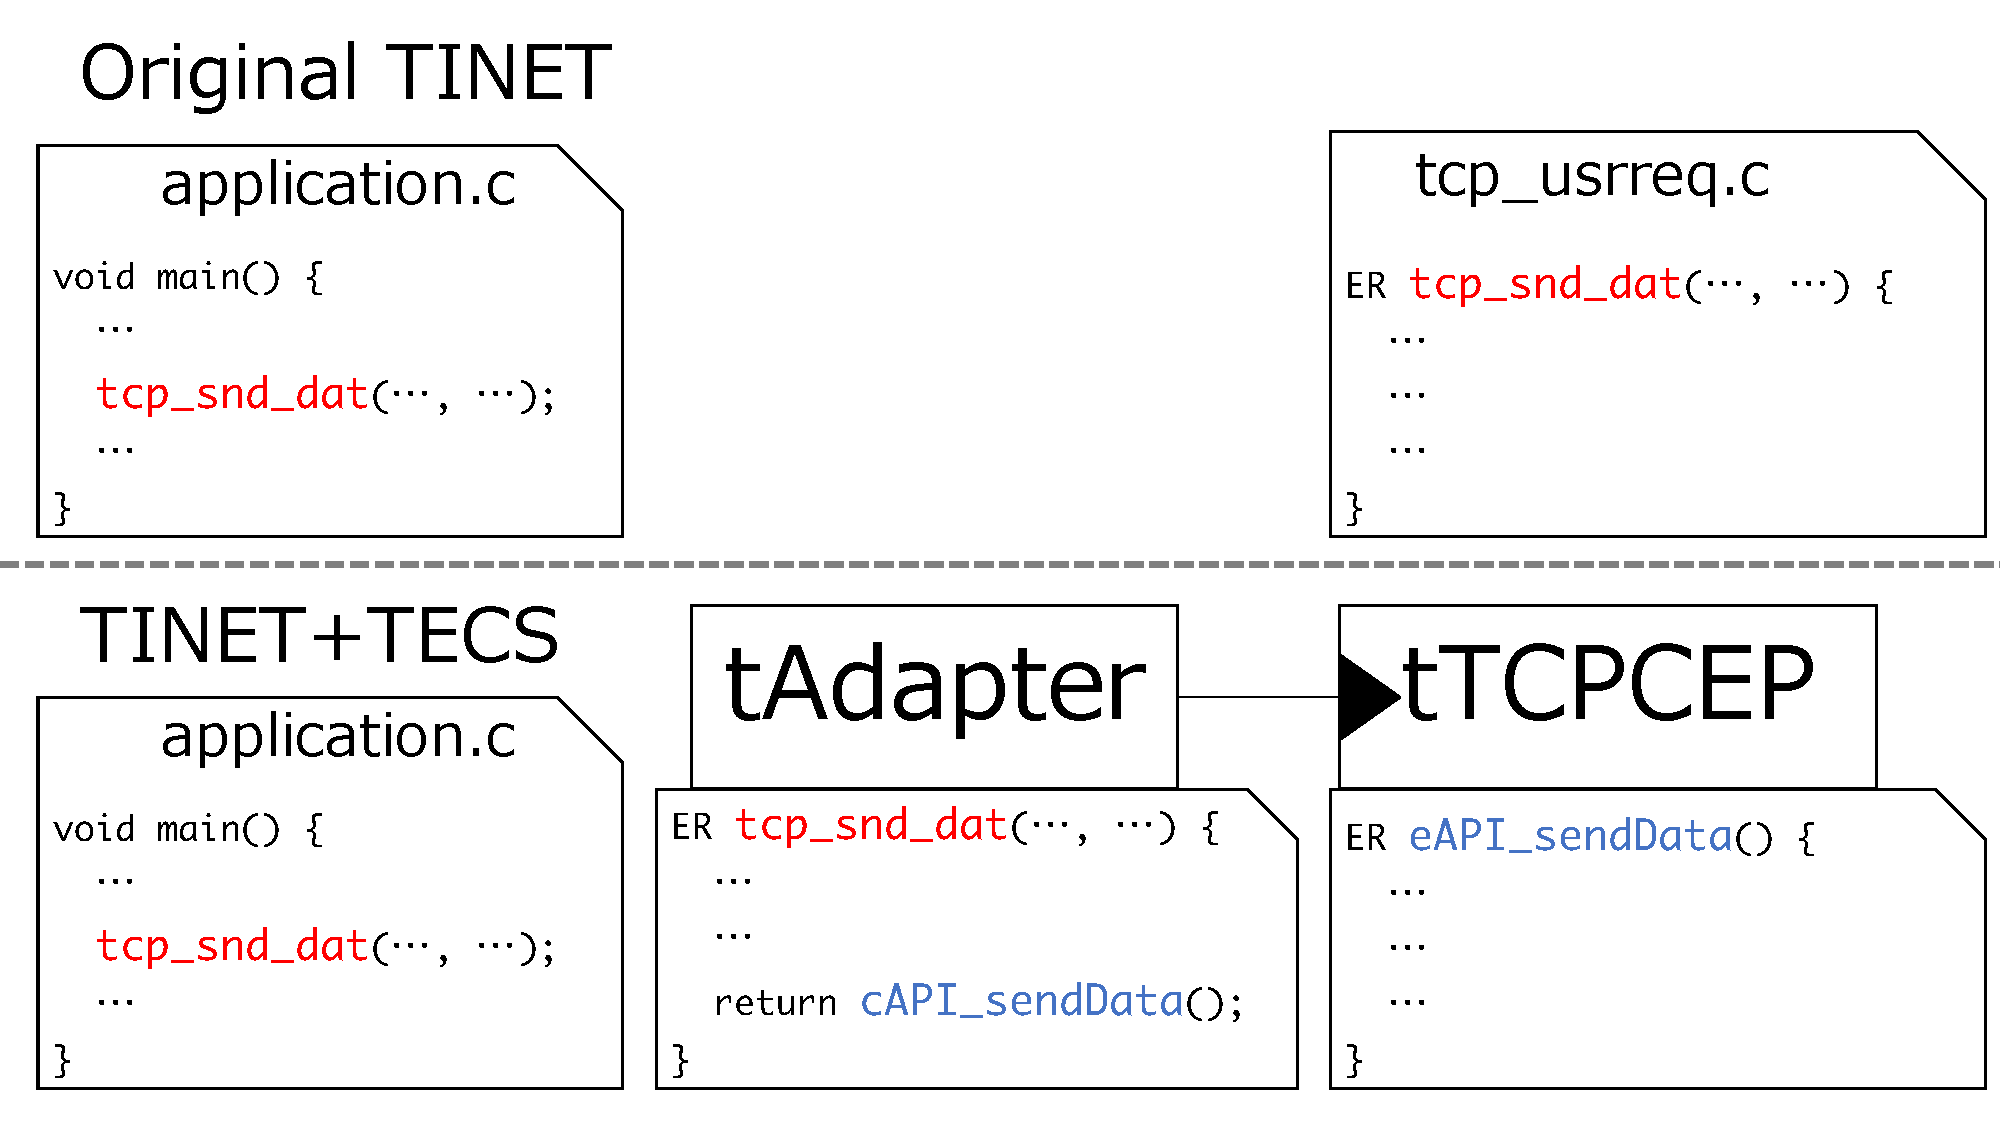
\includegraphics[width=8.0cm,clip]{figure/TECS_Adapter.pdf}
    \caption{TECS adapter}
    \label{fig:TECS_Adapter}
\end{figure}

\section{Evaluation}
\label{sec:Evaluation}

This section describes our experimental evaluation to demonstrate the effectiveness of the proposed framework.

\subsection{Evaluation Environment}

GR-PEACH is employed as the evaluation board.
We connected the board and the host PC with a LAN cable, and evaluated the data transmission and reception.
The detail specification of the board is shown in TABLE \ref{tab:EvaluationBoardEnvironment}.
We also employ TINET 1.5.4 and the compiler arm-none-eabi--gcc 5.2

\begin{table}[t]
    \centering
    \caption{Evaluation Board Environment}
    \begin{tabular}{l|l}
        \hline\hline
        Board           &   GR-PEACH                \\
        CPU             &   Cortex-A9 RZ/A1H 400MHz \\
        Flash ROM       &   8 MB                    \\
        RAM             &   10 MB                   \\
        LAN Controller  &   LAN8710A                \\
        \hline
    \end{tabular}
    \label{tab:EvaluationBoardEnvironment}
\end{table}

\subsection{Performance of TINET+TECS}

To demonstrate the low overhead of TINET+TECS, we evaluated the execution time and the memory consumption of TINET+TECS compared with TINET.

The comparison of execution time between TINET and TINET+TECS is shown in Fig. \ref{fig:EvaluationOfExecutionTime}.
The APIs used for the evaluation are {\it tcp\_snd\_dat} to send TCP data and {\it tcp\_rcv\_dat} to receive TCP data.
For {\it tcp\_snd\_dat}, we measured the executing time from the API calling by the application to the return of the processing result.
In TINET+TECS, the process is performed in the order of tApplication, tTCPCEP, tTCPOutputTaskBody, tIPv4Output, tEthernetOutput, tArp, tEthernetOutputTaskBody, and tIfMbed of Fig. \ref{fig:ComponentProtocolStack}.
For {\it tcp\_rcv\_dat}, we measured the execution time from the data receiving in the LAN driver to the data acquisition in the application.
In TINET+TECS, the process is performed in the order of tIfMbed, tEthernetInputTaskBody, tIPv4Input, tTCPInput, tTCPCEP, and tApplication of Fig. \ref{fig:ComponentProtocolStack}.
The execution time of TINET+TECS is as well as that of TINET; the overhead is about 3 usec.
{\it send/receive} specifiers enable to access the buffer address without data copies.
Therefore, the overhead of componentization does not effect the execution time.

\begin{figure}[t]
    \centering
    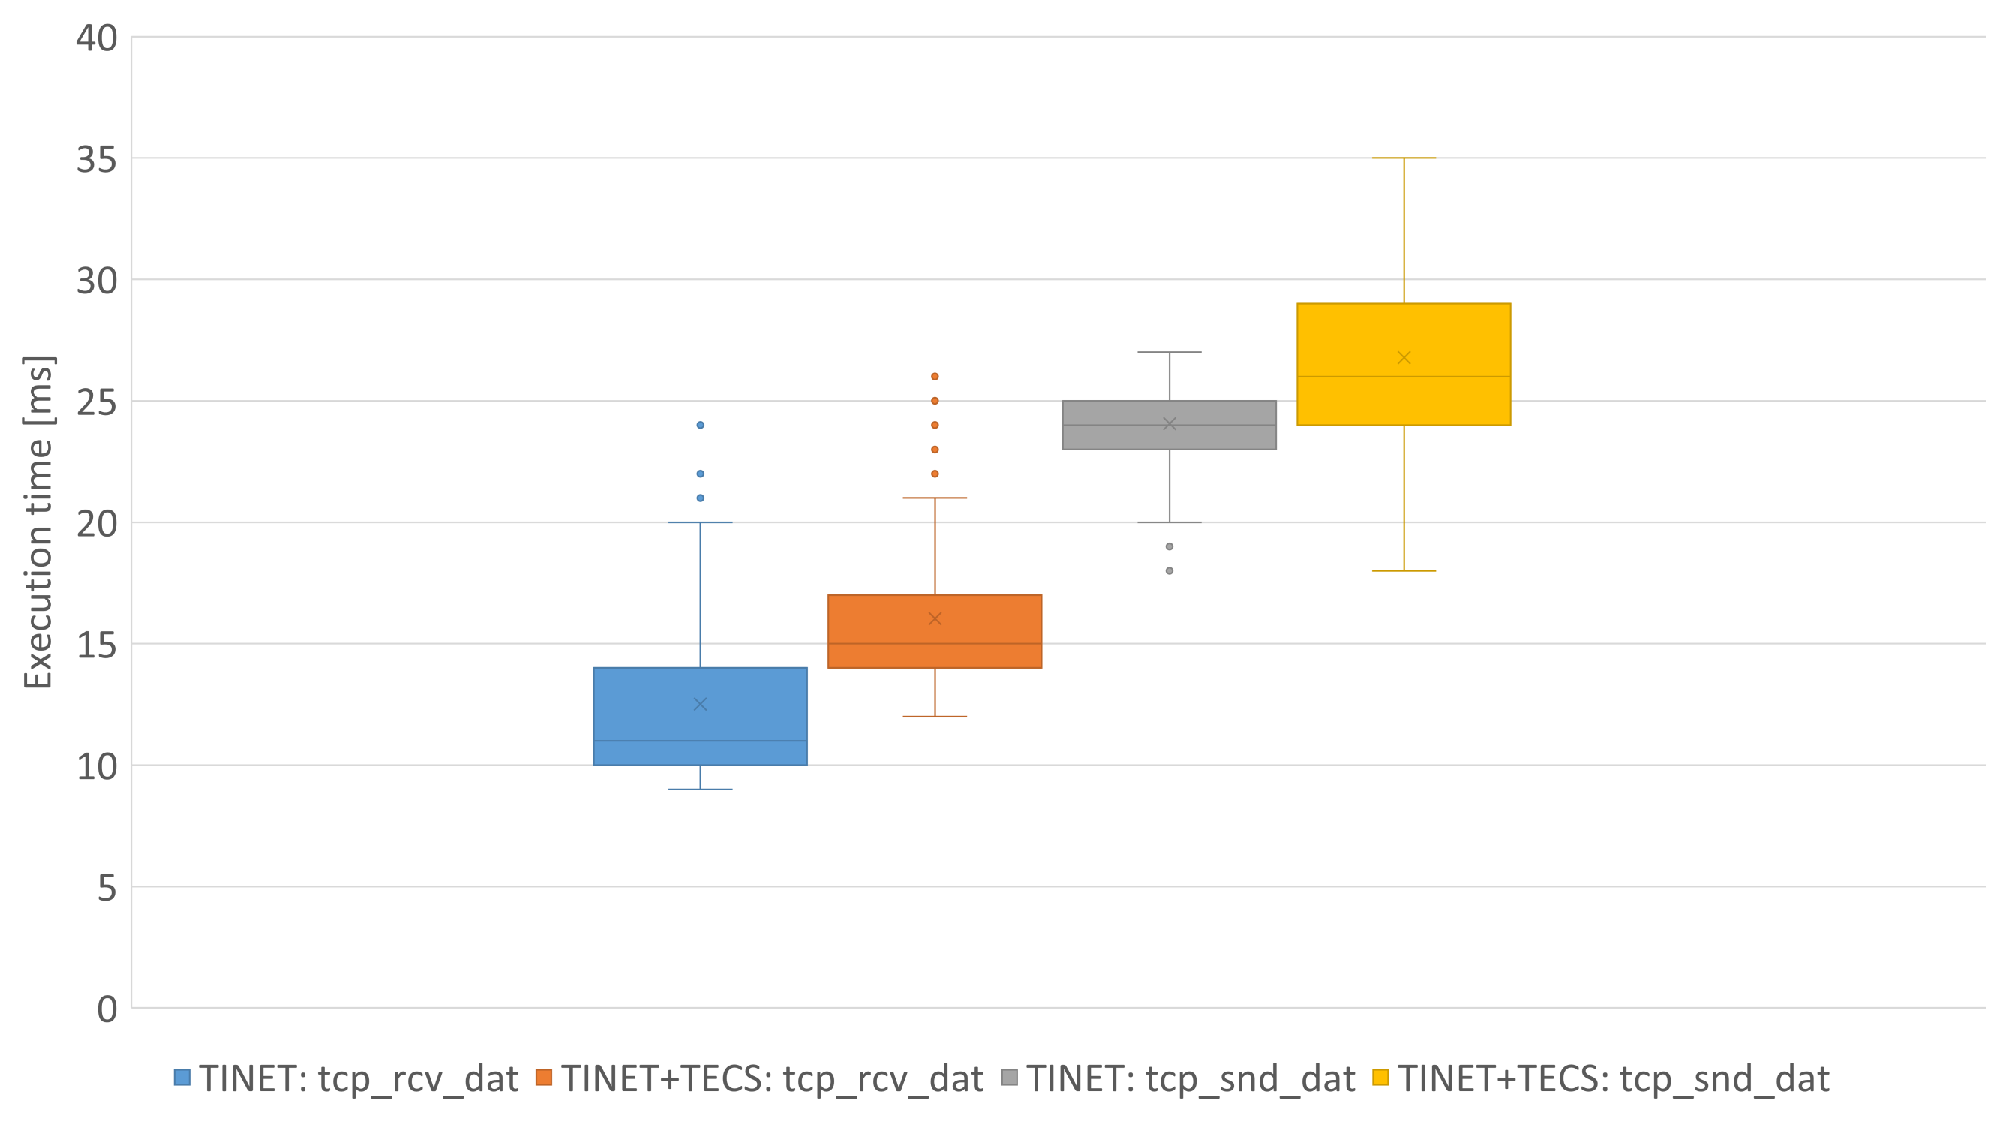
\includegraphics[width=8.0cm,clip]{figure/EvaluationOfExecutionTime.pdf}
    \caption{Execution time of TINET and TINET+TECS}
    \label{fig:EvaluationOfExecutionTime}
\end{figure}

The memory consumptions of TINET and TINET+TECS are compared in TABLE \ref{tab:EvaluationOfMemoryConsumption}.
The memory consumption of TINET+TECS increases about 2.5\% compared with TINET.
The processes and data to manage TECS components, such as initialization of cells, descriptors, function tables, and skeleton functions, cause the increase memory consumption.

\begin{table}[t]
    \centering
    \caption{Memory consumption of TINET and TINET+TECS}
    \begin{tabular}{c|r|r|r|r}
        \hline\hline
                    &   text       &  data    &   bss      &  total     \\ \hline
        TINET       &   183.94 KB  &  5.37 KB &  132.03 KB &  322.34 KB \\
        TINET+TECS  &   170.73 KB  &  5.37 KB &  149.13 KB &  325.23 KB \\
        \hline
        \multicolumn{5}{r}{Including the application and kernel objects}
    \end{tabular}
    \label{tab:EvaluationOfMemoryConsumption}
\end{table}

As shown in TABLE \ref{tab:EvaluationOfConfigurabilty}, the code lines for modification were measured to demonstrate the improved configurability.
We can change the composition of the protocol stack with a small workload.
Thus, the proposed framework improves the configurability.

\begin{table}[t]
    \centering
    \caption{Modified code lines of CDL}
    \begin{tabular}{c|r|r|r}
        \hline\hline
                         &   Size       &   Size (- Default)  & CDL  \\ \hline
        Default          &   325.23 KB  &             0 KB    &  0 lines   \\
        I                &   305.40 KB  &       - 19.83 KB    & 18 lines    \\
        I + I\hspace{-.1em}I &   304.12 KB  &   - 21.10 KB    & 27 lines   \\
        I + I\hspace{-.1em}I + I\hspace{-.1em}I\hspace{-.1em}I & 303.45 KB & - 21.77 KB  & 32 lines \\
        \hline
        \multicolumn{4}{l}{I: Remove TCP}\\
        \multicolumn{4}{l}{I\hspace{-.1em}I: Remove ICMP}\\
        \multicolumn{4}{l}{I\hspace{-.1em}I\hspace{-.1em}I: Change network buffer (Remove memory pools)}
    \end{tabular}
    \label{tab:EvaluationOfConfigurability}
\end{table}


\subsection{Dynamic Connection}

\begin{figure}[t]
    \centering
    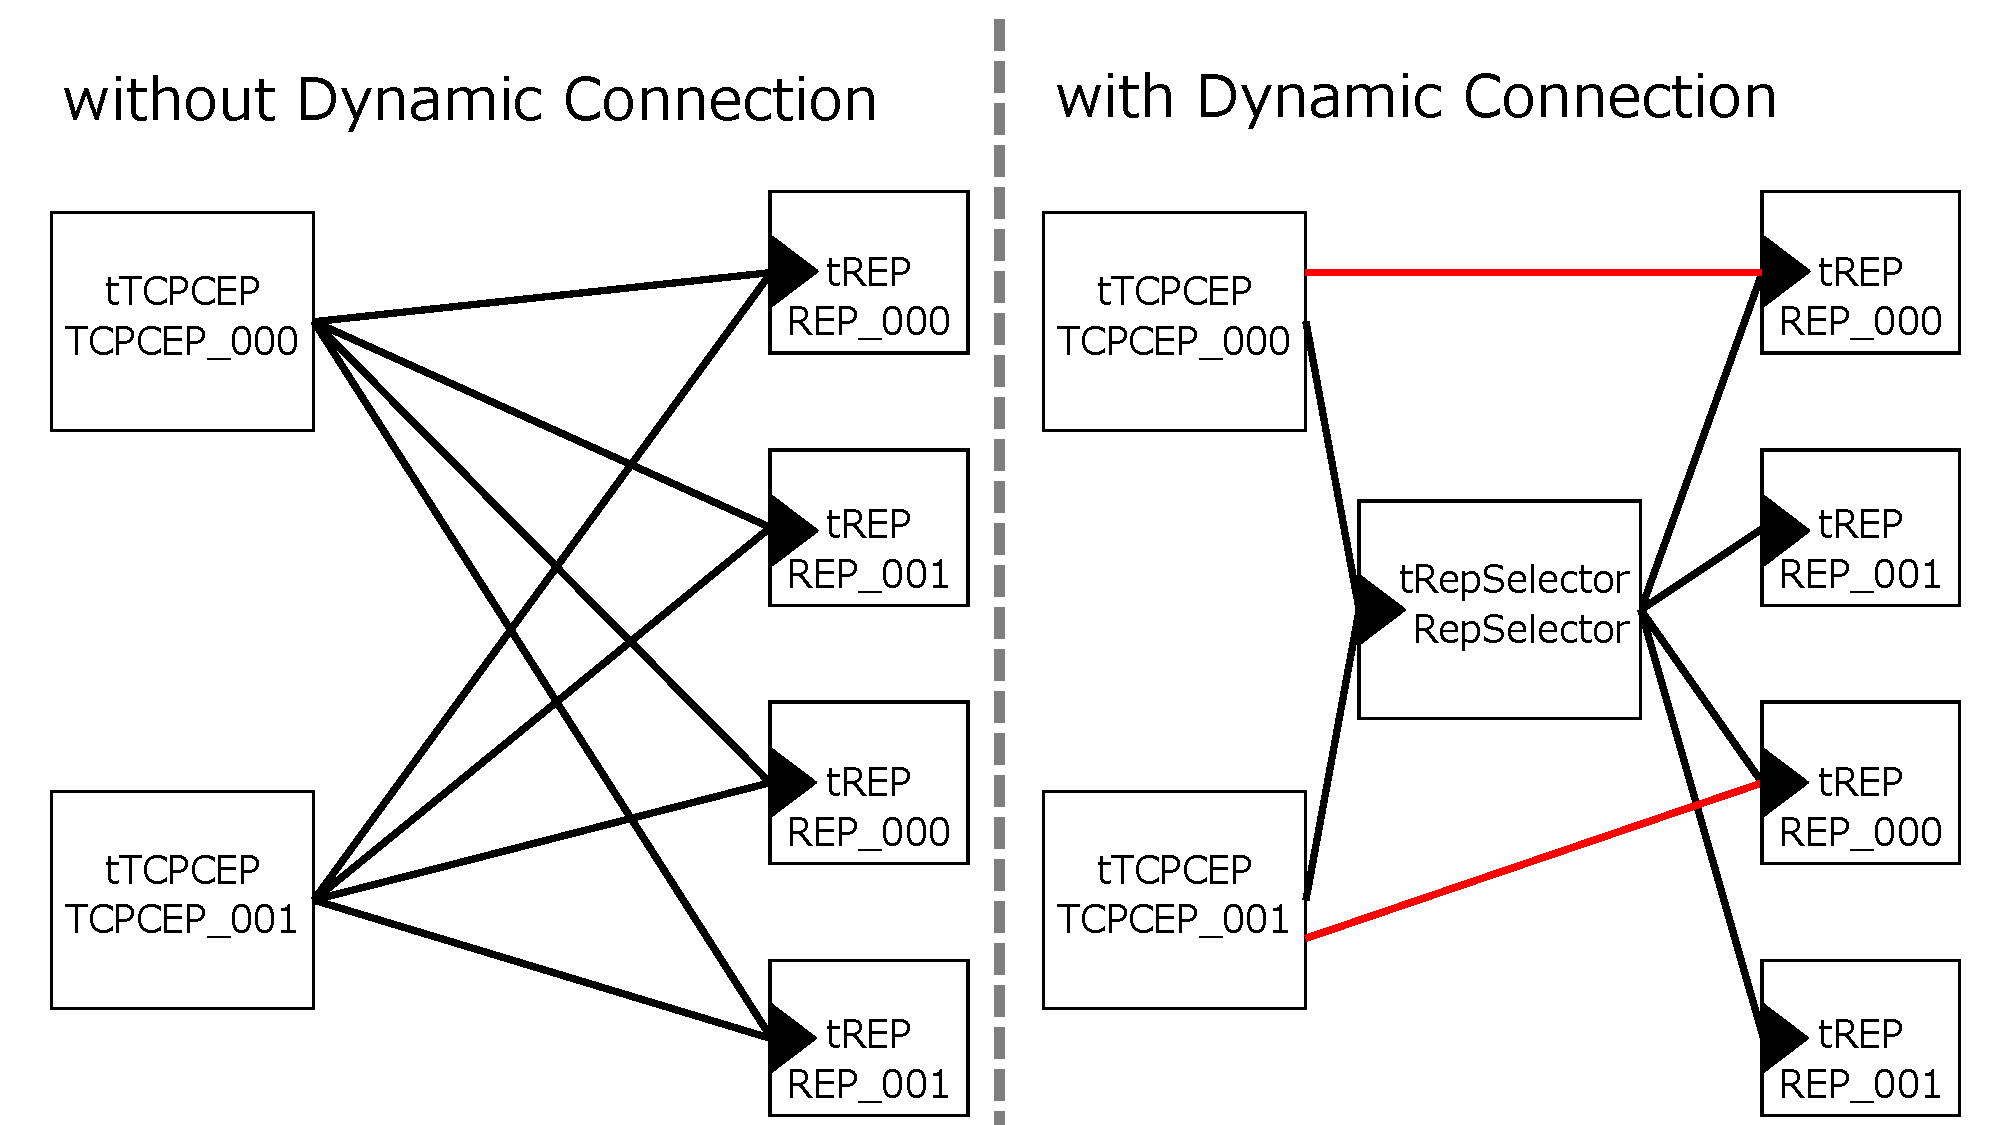
\includegraphics[width=8.0cm,clip]{figure/ComparisonOfDynamicConnection.pdf}
    \caption{Component diagrams of two cases (without/with dynamic connection)}
    \label{fig:ComparisonOfDynamicConnection}
\end{figure}

The memory consumption without and with TECS dynamic connection was evaluated.
As shown in the left of Fig. \ref{fig:ComparisonOfDynamicConnection}, a CEP component should statically connect to all REP components in the case dynamic connection is not used.
As the number of REPs increases, call ports of CEP are required for that.
Thus, it consumes a lot of memory. 
Dynamic connection reduces the memory consumption because only one call port of CEP for REP, which is drawn with red lines in the right of Fig. \ref{fig:ComparisonOfDynamicConnection}, is required per CEP.
Even when the number of REPs increases, a call port of the selector, not the CEP, is joined.

The memory consumption of two cases, without/with dynamic connection, is shown in Fig. \ref{fig:EvaluationOfDynamicConnection}.
The case of dynamic connection consumes the RAM memory more than the other case because the call ports with {\it [dynamic]} is not optimized and allocated in RAM areas as mentioned in Section \ref{sec:DynamicConnection}.
The total memory consumption is fewer in the proposed framework.

\begin{figure}[t]
    \centering
    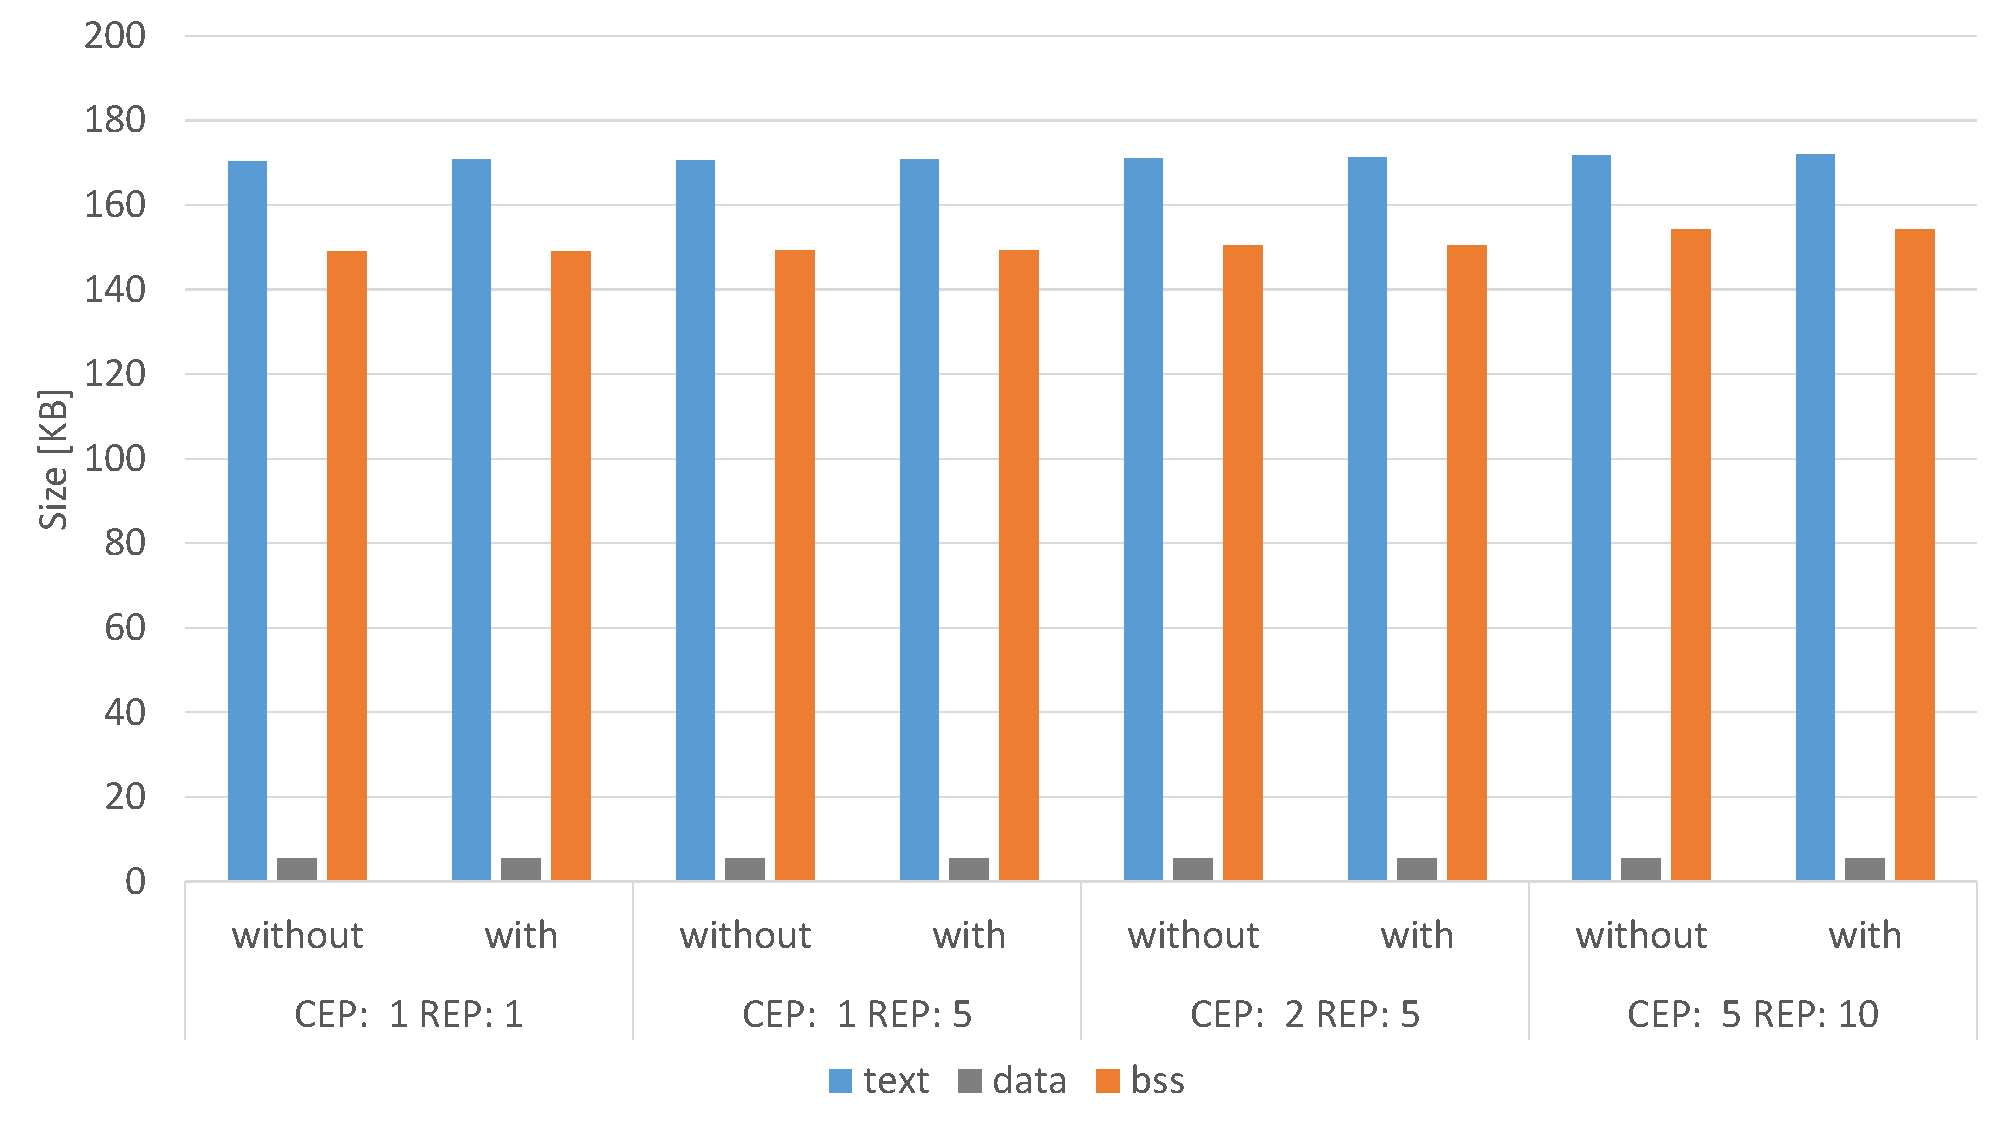
\includegraphics[width=8.0cm,clip]{figure/EvaluationOfDynamicConnection.pdf}
    \caption{Memory consumption of two cases (with/without dynamic connection)}
    \label{fig:EvaluationOfDynamicConnection}
\end{figure}

\begin{table}[t]
    \centering
    \caption{CDL code lines of without/with dynamic connection}
    \begin{tabular}{l|r|r|r}
        \hline\hline
                     &  without  &  with  &  Diff  \\ \hline
        CEP:1 REP:1  &  344 lines     &  347 lines  &  -3 lines   \\
        CEP:1 REP:5  &  369 lines     &  367 lines  &   2 lines   \\
        CEP:2 REP:5  &  387 lines     &  382 lines  &   5 lines   \\
        CEP:5 REP:10 &  485 lines     &  445 lines  &  40 lines   \\
        \hline
    \end{tabular}
    \label{tab:EvaluationOfConfigurabilityByDynamicConnection}
\end{table}

\begin{figure}[t]
 \centering
 \begin{lstlisting}
/* without Dynamic Connection */
cell tTCPCEP TCPCEP_000 {
    cREP[0] = REP_000.eREP;
    ..
    cREP[n] = REP_00n.eREP;
};
cell tTCPCEP TCPCEP_001 {
    cREP[0] = REP_000.eREP;
    ..
    cREP[n] = REP_00n.eREP;
};
..
cell tTCPCEP TCPCEP_00n {
    cREP[0] = REP_000.eREP;
    ..
    cREP[n] = REP_00n.eREP;
};
 \end{lstlisting}
 \centering
 \begin{lstlisting}
/* with Dynamic Connection */
cell tRepSelector RepSelector {
    cREP[0] = REP_000.eREP;
    ..
    cREP[n] = REP_00n.eREP;
};
cell tTCPCEP TCPCEP_000 {
    cRepSelector = RepSelector.eRepSelector;
};
cell tTCPCEP TCPCEP_001 {
    cRepSelector = RepSelector.eRepSelector;
};
..
cell tTCPCEP TCPCEP_00n {
    cRepSelector = RepSelector.eRepSelector;
};
 \end{lstlisting}
 \caption{Comparison of CDL descriptions between without/with dynamic connection}
 \label{src:ComparisonOfCDL}
\end{figure}

The comparison of CDL code lines of without/with dynamic connection is shown in TABLE \ref{tab:EvaluationOfConfigurabilityByDynamicConnection}, to demonstrate improved configurability by dynamic connection.
As the number of CEPs and REPs increases, the amount of CDL code lines to be added increases.
In the left part of Fig. \ref{fig:ComparisonOfDynamicConnection}, each CEP connects all REPs as shown in the upper of Fig. \ref{src:ComparisonOfCDL}. 
In the right part of Fig. \ref{fig:ComparisonOfDynamicConnection}, a CEP dynamically connects an REP, and only the selector connects all REPs as shown in the lower of Fig. \ref{src:ComparisonOfCDL}. 
Since the difference spreads as the number of CEPs and REPs increases, it is effective for software that uses many ports.


\subsection{Overhead of Adapter}

The execution time of API with the adapter such as {\it tcp\_snd\_dat/eAPI\_sendData} to analyze the overhead of TECS adapter which supports existing applications.
As shown in Fig. \ref{fig:EvaluationOfAdapter}, the overhead of TECS adapter is very small because the adapter only passes the parameters to TECS components from C codes.
Therefore, TECS adapter does not affect the system.

\begin{figure}[t]
    \centering
    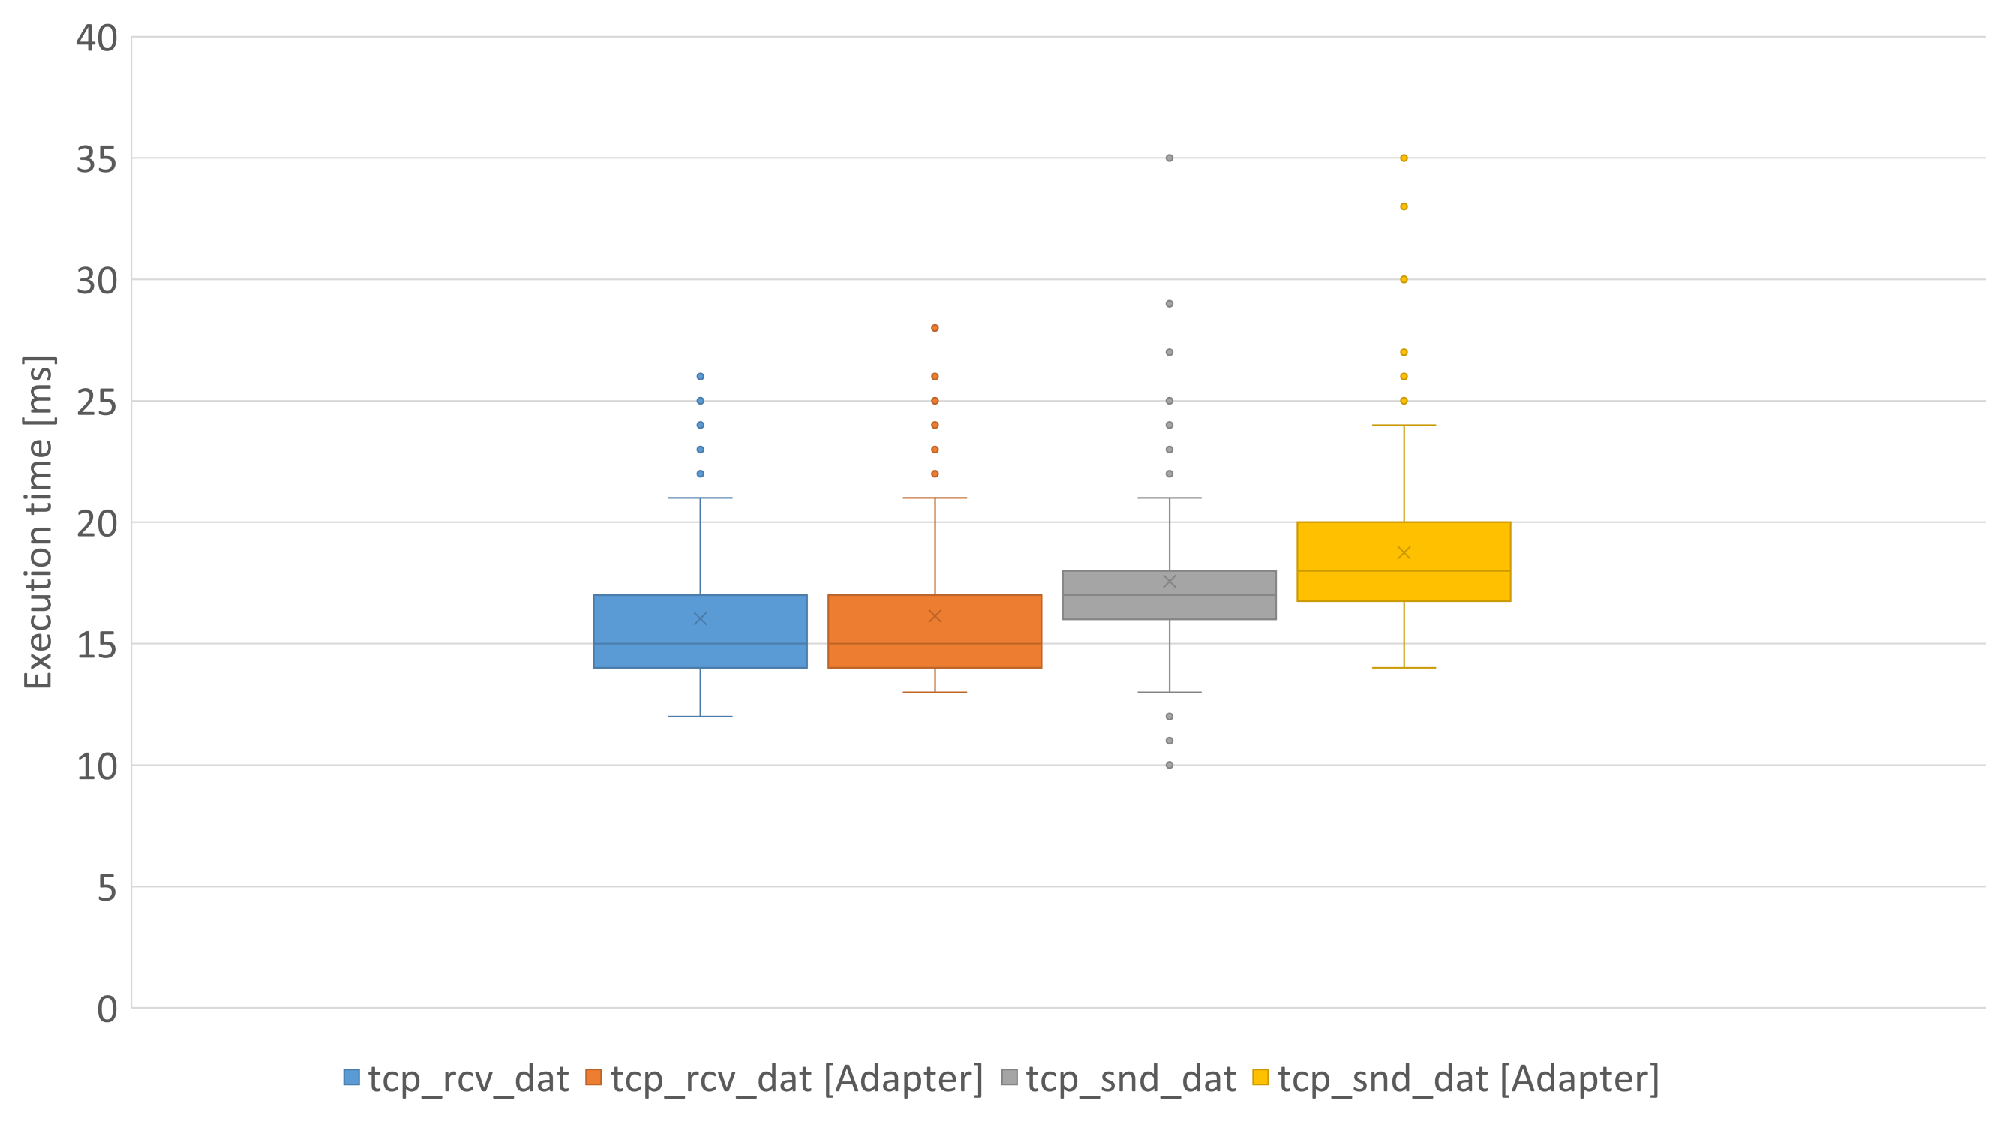
\includegraphics[width=8.0cm,clip]{figure/EvaluationOfAdapter.pdf}
    \caption{Execution time of two cases (without/with TECS adapter)}
    \label{fig:EvaluationOfAdapter}
\end{figure}


\section{Related Work}
\label{sec:Related Work}

Open-source TCP/IP protocol stacks for embedded systems have been developed such uIP \cite{par:uIP}, lwIP \cite{par:lwIP}.

{\bf uIP:}
uIP (microIP) is a very small TCP/IP stack intended for tiny 8-bit and 16-bit microcontrollers.
    uIP only requires about five KB of code size and several hundreds bytes of RAM.
uIP has been ported to various systems and has found its way into many commercial products.
After ver. 1.0 is released, later versions of uIP, including uIPv6, are integrated with Contiki OS \cite{par:Contiki},\cite{url:Contiki}, an operating system to connect tiny microcontroller to the Internet.

{\bf lwIP:}
lwIP (lightweightIP) is a small TCP/IP implementation for embedded systems.
The focus of lwIP is to reduce memory resource while still having a full scale TCP.
lwIP requires about 40 KB of ROM and tens of KB of RAM.
lwIP is larger than uIP, but provides better throughput.

% {\bf CiAO/IP:}
% \\
% \\
% Should be written
% \\
% \\

\section{Conclusion}
\label{sec:Conclusion}

This paper proposed TINET+TECS, a component-based TCP/IP protocol stack for embedded systems.
TINET+TECS is componentized TINET, which is a compact TCP/IP protocol stack, using TECS.
TINET consists of many macros and complicated codes and the software productivity are low.
The proposed framework improves the configurability while suppressing the overhead of componentization.
The proposed framework also improves the scalability because the component-based framework simplifies to add/remove and change protocols such as TCP/UDP, IPv4/IPv6, and Ethernet/PPP.

In addition, this paper presents dynamic connection, a new method of TECS, to enable dynamic processing while reducing memory consumption.
To satisfy TINET specification that TINET support static generation of CEPs and REPs, TINET+TECS utilizes dynamic connection.
TECS adapter supports legacy codes, existing TCP/IP applications can run without modification in the proposed framework.

In the future, the proposed framework will cooperate with mruby on TECS \cite{par:mrubyonTECS} to easily manage IoT devices.
Note that mruby is a scripting language for embedded systems \cite{par:mruby}.
We will support the functionalities that TINET functions can be utilized from mruby programs as an extension of mruby-socket \cite{url:mruby-library}.

    
% conference papers do not normally have an appendix


% use section* for acknowledgment
\section*{Acknowledgment}

The authers would like to thank Hiroaki Nagashima for supporting this research.
This work is supported by JSPS KAKENHI Grant Number 15H05305.

% trigger a \newpage just before the given reference
% number - used to balance the columns on the last page
% adjust value as needed - may need to be readjusted if
% the document is modified later
%\IEEEtriggeratref{8}
% The "triggered" command can be changed if desired:
%\IEEEtriggercmd{\enlargethispage{-5in}}

% references section
\bibliographystyle{IEEEtranBST2/IEEEtran}
\bibliography{ref}

% that's all folks
\end{document}
